\documentclass[times, utf8, zavrsni, numeric]{fer}
\usepackage{booktabs}
\usepackage{graphicx}
\usepackage{subcaption}
\usepackage{gensymb}
\usepackage{indentfirst}
\usepackage{amssymb}
\usepackage{commath}
\usepackage{hyperref} 

\begin{document}

\thesisnumber{5187}
\title{Ekstrakcija tablica na skeniranim dokumentima}
\author{Kristijan Vulinović}

\maketitle

% Ispis stranice s napomenom o umetanju izvornika rada. Uklonite naredbu \izvornik ako želite izbaciti tu stranicu. 
\izvornik

% Dodavanje zahvale ili prazne stranice. Ako ne želite dodati zahvalu, naredbu ostavite radi prazne stranice.
\zahvala{Zahvaljujem svima onima koji su dio svojeg vremena odvojili kako bi ispunili primjerke tablica, kao i svima koji su pomogli prilikom prikupljanja istih.}

\tableofcontents

\chapter{Uvod   }
U današnje vrijeme postoje izuzetno velike količine papirnatih dokumenata.
Samo u Sjedinjenim Američkim Državama nastaje više od milijarde novih papirnatih dokumenata svakog radnog dana. 
Mogućnost digitalizacije takvih dokumenata može biti od velike koristi prilikom pohrane, slanja ili pretraživanja istih \cite{article:Skew-detection}.
Digitalizaciju dokumenata možemo podijeliti u dva dijela: prepoznavanje teksta te prepoznavanje grafičkih objekata \cite{conference:DetectionOfTableStructure}. 
Za prepoznavanje teksta dostupan je velik broj alata koji omogućuju optičko prepoznavanje znakova (engl. \textit{optical character recognition}).
Prepoznavanje grafičkih objekata dokumenta mnogo je manje zastupljeno u odnosu na prepoznavanje teksta te je postalo popularnije tek u novije vrijeme. 
U to spada prepoznavanje linija, oblika, slika, simbola, tablica i raznih drugih objekata koji se mogu nalaziti na skeniranim dokumentima.
Intenzivan razvoj ovoga područja nastupio je zahvaljujući razvoju dubokih neuronskih mreža i sklopovlja koje omogućuje velike brzine izračuna koje prije nisu bile moguće.\\

Ovaj rad se fokusira isključivo na prepoznavanje tablica, što je prethodno već opisano u radovima poput \cite{conference:DetectionOfTableStructure} i \cite{conference:AutomaticTableDetectionInDocumentImages}. 
Taj postupak se dijeli na prepoznavanje položaja tablice u odnosu na ostatak dokumenta, prilikom čega je potrebno u dokumentu izdvojiti tablicu od ostatka teksta i ostalih grafičkih objekata, a što je opisano u radu \cite{article:Medium-IndependentTableDetection}.
Nakon što je tablica pronađena određuje se njezin izgled, tako da se odredi broj redaka i stupaca, a potom koordinate pojedine ćelije.
Postupak je detaljnije opisan u nastavku rada. \\

U radu \cite{article:Medium-IndependentTableDetection} je opisan postupak u kojemu se tablice prepoznaju na temelju praznog prostora koji ih okružuje, odnosno pomoću praznog prostora između redaka i stupaca kod tablica koje nemaju crte. Fokus rada je na prepoznavanju ASCII tablica. Rad \cite{article:SimpleAndEffectiveTableDetectionSystemFromDocumentImages} također se zasniva na sličnom principu, uz razliku da je namijenjen općenitim dokumentima te prepoznaje tablice s crtama, što radi tako da mjeri udaljenosti između teksta koje se razlikuju od standardnih udaljenosti znakova u riječima.
U radu \cite{LayoutRecognitionofTable-Form} predstavljena je metoda koja detekciju tablice obavlja u $2$ koraka.
Najprije se generira stablo strukture dokumenta, što omogućava prepoznavanje tablica bilo kakvog oblika, a ne nužno samo standardnih kvadratnih tablica, nakon čega se vrši ekstrakcija sadržaja ćelija kako bi se isti dodatno obradio.
Rad \cite{conference:AutomaticTableDetectionInDocumentImages} opisuje postupak detekcije tablica na temelju obrade slike te prepoznavanju pozicija linija i njihovih sjecišta.
Na taj se način određuju vrhovi ćelija iz čega se rekonstruira tablica, te je postignuto prepoznavanje tablica bez prethodnog procesa učenja.
\\

Predstavljeno rješenje počinje od slike u sivim tonovima (engl. \textit{gray-scale}), koja se binarizira kako bi se dobila slika koja se sastoji od isključivo crne i bijele boje.
Dobivena crno-bijela slika koristi se u daljnjoj obradi te se provjerava je li slika rotirana, odnosno kut rotacije iste, nakon čega se slika po potrebi rotira kako bi tablica stajala okomito.
Ovako obrađena slika koristi se dalje za detekciju tablica, postupkom koji se temelji na prepoznavanju kuteva ćelija korištenjem klasifikatora temeljenog na algoritmu AdaBoost i klasifikatora primjenom umjetne neuronske mreže.
Prepoznati uglovi ćelija kasnije se rekonstruiraju u tablicu, a što je detaljno opisano u nastavku rada.

Ostatak ovog rada organiziran je kako slijedi.
U poglavlju \ref{ch:binarization} objašnjen je postupak binarizacije slike.
Objašnjena su $2$ različita postupka te su opisane prednosti i mane svakoga.
Poglavlje \ref{ch:skewDetection} objšnjava postupak određivanja rotiranosti početne slike i ispravljanja prepoznate rotacije.
Detekcija tablice objašnjena je u poglavlju \ref{ch:tableDetection}.
U istom poglavlju objašnjeno je prikupljanje značajki na temelju kojih se tablice prepoznaju, kao i rad umjetnih neuronskih mreža i algoritam AdaBoost koji su korišteni u svrhu prepoznavanja.
U poglavlju \ref{ch:implementation} objašnjena je implementacija algoritama iz poglavlja \ref{ch:tableDetection} te je objašnjen način rada genetskih algoritama i algoritma propagacije pogreške unatrag koji su korišteni prilikom treniranja neuronske mreže.


\chapter{Binarizacija slike}
\label{ch:binarization}
Početna slika dana je kao crno-bijela slika koja sadrži $256$ nijansi sive boje, gdje je crna označena s vrijednošću $0$, a bijela s $255$.
Prije nego li se započne bilo kakva analiza slike, potrebno je istu binarizirati, odnosno pretvoriti u oblik koji će sadržavati isključivo crne ili bijele elemente, bez ostalih nijansi sive.
To je moguće učiniti na dva načina: korištenjem fiksno definiranog praga nakon kojega ćemo svaku vrijednost proglasiti crnom, ili korištenjem adaptivne binarizacije koja se temelji na usporedbi trenutnog intenziteta sive s intenzitetom sive u okruženju.

\section{Binarizacija fiksnim pragom}
Najjednostavniji oblik binarizacije je korištenje fiksno definiranog praga.
U tom se slučaju gleda svaki pojedini slikovni element te ako je njegova vrijednost manja od zadanog praga, element se postavlja na crnu boju, dok se u protivnom postavlja na bijelu.
Prednosti ove metode su izrazito jednostavna implementacija, ali i velika brzina izvođenja. 
Nedostatci se primjećuju u slučajevima lošeg ili nejednolikog osvjetljenja gdje se događa da se neki dijelovi dokumenta u potpunosti prepoznaju kao crni, unatoč činjenici da je prethodno bilo moguće razlikovati i prepoznati pozadinu od sadržaja dokumenta.
Slika \ref{fig:threshold} prikazuje opisani problem te se na istoj može primijetiti kako je u donjem lijevom kutu slike tamno područje, koje nakon binarizacije postaje u potpunosti crno. 
Također se primjećuje i kako je gornji desni kut slike slabije osvijetljen, zbog čega u binariziranoj slici slova postaju tanja i slabije vidljiva.\\

\begin{figure}[th!]
    \centering
    \begin{subfigure}{.5\textwidth}
        \centering
        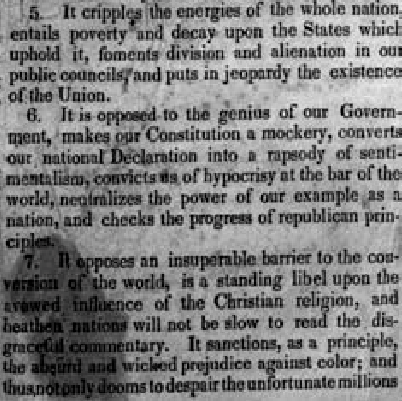
\includegraphics[width=.85\linewidth]{Images/Grayscale.png}
        \captionsetup{justification=centering}
        \caption{Početna crno-bijela slika (slika je preuzeta iz \cite{AdaptiveBinarization})}
        \label{fig:sub1}
    \end{subfigure}%
    \begin{subfigure}{.5\textwidth}
        \centering
        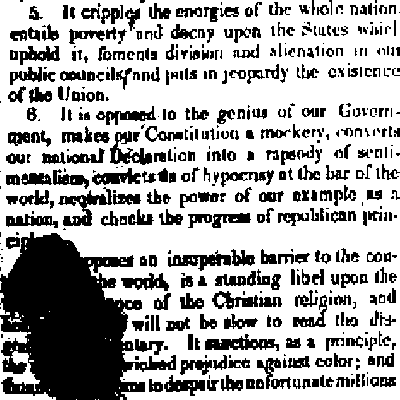
\includegraphics[width=.85\linewidth]{Images/Threshold.png}
        \caption{Slika dobivena binarizacijom fiksnim pragom}
        \label{fig:sub2}
    \end{subfigure}
    \caption{Primjer binarizacije fiksnim pragom}
    \label{fig:threshold}
\end{figure}

\section{Adaptivna binarizacija}
Problemi prikazani u prethodnom postupku rješavaju se primjenom adaptivne binarizacije koja vrijednost svakog pojedinog slikovnog elementa ne određuje samo na osnovu njegove boje, već u obzir uzima i boju okoline.
U nastavku je opisan postupak koji je predložen u \cite{AdaptiveBinarization}.
Prikazani primjeri koriste sliku \ref{fig:sub1} kao početnu.

\subsection{Filtriranje šuma}
Ovisno o stanju dokumenta i načinu digitalizacije istoga moguće je da se na dobivenoj slici pojavljuje šum, kojega je potrebno otkloniti.
Za potrebe opisanoga koristi se Wienerov niskopropusni filter \cite{book:Two-Dimensional-Signal-Image-Processing}, koji radi na principu statističke procjene intenziteta slikovnog elementa temeljene na okruženju svakog pojedinog slikovnog elementa \cite{AdaptiveBinarization}.
Označimo s $I_s(x, y)$ vrijednost slikovnog elementa početne slike, a s $I(x, y)$ vrijednost slikovnog elementa filtrirane slike.
Tada se filtrirana slika $I$ može izračunati pomoću izraza opisanog u knjizi \cite{book:Two-Dimensional-Signal-Image-Processing}:
\[I(x, y) = \mu(x, y) + \frac{\sigma(x, y)^2}{(\sigma(x, y)^2 - v^2)}(I_s(x, y) - \mu(x, y)).\]
$\mu(x, y)$ označava je aritmetičku sredinu vrijednosti intenziteta slikovnih elemenata u okruženju veličine $N\times M$, prema izrazu:
\[\mu(x, y) = \frac{1}{NM} 
    \displaystyle \sum_{i = x-\frac{N}{2}}^{x+\frac{N}{2}}
    \displaystyle \sum_{j = y-\frac{M}{2}}^{y+\frac{M}{2}}
I_s(i, j),\]
gdje $\sigma^2$ označava varijancu vrijednosti intenziteta slikovnih elemenata u okruženju veličine $N\times M$, prema izrazu:
\[\sigma(x, y)^2 = \frac{1}{NM} 
    \displaystyle \sum_{i = x-\frac{N}{2}}^{x+\frac{N}{2}}
    \displaystyle \sum_{j = y-\frac{M}{2}}^{y+\frac{M}{2}}
(I_s(i, j)^2 - \mu^2).\]
$v^2$ označava srednju vrijednost svih lokalnih varijanci.
Konačan rezultat filtriranja, korištenjem okruženja dimenzija $5\times 5$ prikazan je na slici \ref{fig:wiener}.

\begin{figure}[!ht]
\centering
\begin{minipage}{.5\textwidth}
    \centering
    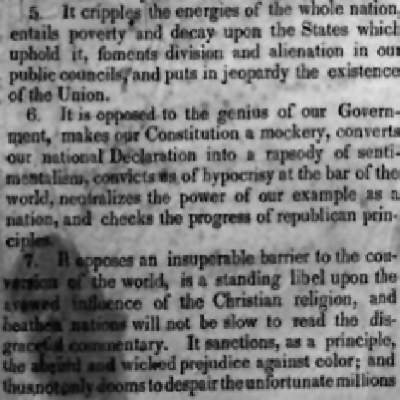
\includegraphics[width=.85\linewidth]{Images/Wiener.png}
    \caption{Slika dobivena filtriranjem šuma}
    \label{fig:wiener}
\end{minipage}%
\begin{minipage}{.5\textwidth}
    \centering
    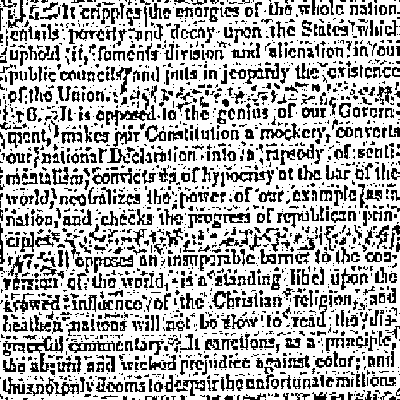
\includegraphics[width=.85\linewidth]{Images/Niblack.png}
    \captionsetup{justification=centering}
    \caption{Slika dobivena korištenjem Niblackovog algoritma adaptivne binarizacije}
    \label{fig:niblack}
\end{minipage}
\end{figure}

\subsection{Procjena sadržaja}
Sljedeći korak binarizacije temelji se na procjenjivanju sadržaja dokumenta. 
Cilj ovog koraka je procijeniti koji elementi slike pripadaju pozadini, a koji pripadaju sadržaju dokumenta. 
Pritom je procijenjeni sadržaj zapravo nadskup stvarnog sadržaja, odnosno na dobivenoj slici bit će prisutan šum. 
Za potrebe ovoga koristi se Niblackov algoritam adaptivne binarizacije \cite{AdaptiveBinarization}.\\

Algoritam se temelji na ideji kliznog prozora (engl. \textit{sliding window}) određenih dimenzija, pomoću kojega se računa lokalni medijan  $m$ te varijanca $s$. 
Kako bi se ubrzao izračun, umjesto medijana se računa aritmetička sredina $\mu$.
Konačan prag binarizacije, $T$, određuje se kao:
\[ T = m + ks,\]
gdje je $k$ proizvoljna konstanta koja određuje koliko će okolina trenutnog slikovnog elementa utjecati na prag binarizacije.
Korištena vrijednost je $k = -0.2$.
Konačna slika $N$, dobivena je od početne slike $I$ na sljedeći način:
\[
    N(x, y) =
    \begin{cases}
        1,   & \quad \text{ako je } I(x, y) > T\\
        0,  & \quad \text{inače}.\\
    \end{cases}
\]
Rezultati ovog postupka, korištenjem kliznog prozora dimenzija $20$x$20$, uz $k=-0.2$, prikazan je na slici \ref{fig:niblack}.
Na slici se primjećuje kako je sav tekst prepoznat i prikazan crnom bojom, ali je također prisutan i jako izražen šum.

\subsection{Procjena pozadine}
U ovom koraku pokušava se procijeniti izgled pozadine dokumenta, što je označeno sa $B$. 
Za potrebe toga koristi se obrađena početna slika $I$ te prethodno dobivena slika $N$.
Ako je neki slikovni element na slici $N$ označen nulom, taj element predstavlja pozadinu slike i njegova vrijednost na slici $B$ bit će jednaka onoj sa slike $I$.
U protivnome će vrijednost tog slikovnog elementa biti određena interpolacijom vrijednosti susjednih slikovnih elemenata.
Konačan izraz za elemente slike $B$ glasi:
\[
    B(x, y) =
    \begin{cases}
        \hfil
        I(x, y),    & \quad \text{ako je } N(x, y) = 0\\[1em]
        \frac{
            \displaystyle \sum_{i = x-dx}^{x+dx}
            \displaystyle \sum_{j = y-dy}^{y+dy}
            (I(i, j)(1 - N(i, j)))
        } {
            \displaystyle \sum_{i = x-dx}^{x+dx}
            \displaystyle \sum_{j = y-dy}^{y+dy}
            (1 - N(i, j))
        }, & \quad \text{ako je} N(x, y) = 1.\\

    \end{cases}
\]
Pri čemu $dx$ i $dy$ određuju dimenzije okruženja koje se gleda prilikom interpolacije.
Postupak je u cijelosti objašnjen u radu \cite{AdaptiveBinarization}.\\

\begin{figure}[!ht]
\centering
\begin{minipage}{.5\textwidth}
    \centering
    
\includegraphics[width=.85\linewidth]{Images/Background.png}
    \caption{Slika dobivena procjenom pozadine}
    \label{fig:background}
\end{minipage}%
\begin{minipage}{.5\textwidth}
    \centering
    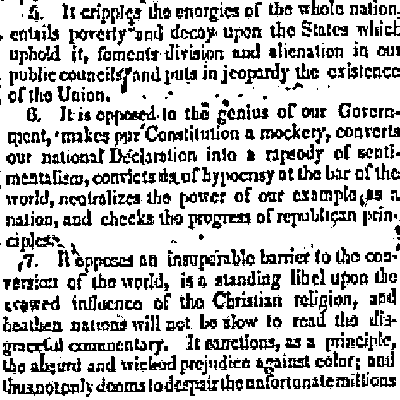
\includegraphics[width=.85\linewidth]{Images/FinalThreshold.png}
    \captionsetup{justification=centering}
    \caption{Slika dobivena binarizacijom}
    \label{fig:finalThreshold}
\end{minipage}
\end{figure}

Rezultati ovog postupka, primijenjenog  na slici \ref{fig:sub1} prikazani su na slici \ref{fig:background}, uz $dx=3$ i $dy=3$.
Moguće je uočiti kako se na slici i dalje primjećuju obrisi slova, premda sama slova nisu prisutna.

\subsection{Binarizacija}
Kao što je opisano u radu \cite{AdaptiveBinarization}, u ovom koraku se provodi konačna binarizacija, uspoređivanjem izračunate pozadine $B$ i izvorne slike $I$.
Postupak se temelji na tome da je razlika u boji teksta i pozadine veća nego li razlika u boji šuma dobivenog procjenom sadržaja dokumenta i pozadine.
Ovisno o intenzitetu sive boje okruženja, računa se prag binarizacije $d$, kako bi se sačuvao tekst u tamnim područjima.
Kako bi se to postiglo, vrijednost praga $d$ mora biti manja u područjima s tamnom pozadinom.
Konačna slika $T$ određena je izrazom:
\[
    T(x, y) = 
    \begin{cases}
    1,  & \quad \text{ako je } B(x, y) - I(x, y) > d(B(x, y)) \\
    0,  & \quad \text{inače}.\\
    \end{cases}
\]
Vrijednost praga, $d(B(x, y))$, moguće je procijeniti kao 
\[d = q \cdot \delta\]
gdje je $q$ konstanta koja je fiksno postavljena na $0.8$, a $\delta$ se računa kao razlika intenziteta sive boje na početnoj slici za mjesta koja predstavljaju pozadinu i za mjesta koja predstavljaju tekst.
Vrijednost $\delta$ možemo aproksimirati kao
\[
    \delta = \frac{
        \displaystyle \sum_x
        \displaystyle \sum_y
        (B(x, y) - I(x, y))
    }{
        \displaystyle \sum_x
        \displaystyle \sum_y
        N(x, y)
    }.
\]

Konačan rezultat nakon primjene opisanog postupka binarizacije prikazan je na slici \ref{fig:finalThreshold}.
Za razliku od rezultata korištenjem binarizacije s fiksnim pragom, prikazanim na slici \ref{fig:sub2}, primjećuje se kako zatamnjeno područje u donjem lijevom kutu slike ne predstavlja problem prilikom raspoznavanja teksta od pozadine.
Također je potrebno primijetiti i šumove koji su ostali prisutni nakon trenutno opisanog postupka, a koji su riješeni u nastavku.

\subsection{Dodatna obrada slike}
Završni korak obrade slike koristi se kako bi se popravila kvaliteta konačne binarizirane slike.
Problemi koji se mogu uočiti na danim primjerima uključuju prisutnost šuma, kao i potencijalne prekide slova, gdje je moguće da neko slovo nije u potpunosti zacrnjeno.\\

\begin{figure}[!ht]
\centering
\begin{minipage}{.5\textwidth}
    \centering
    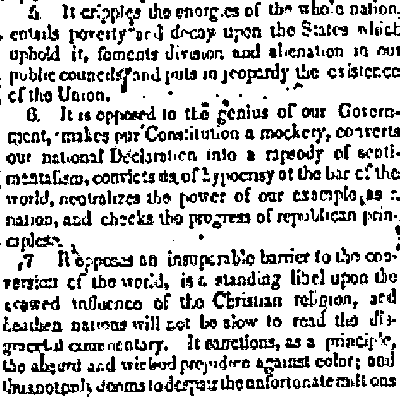
\includegraphics[width=.85\linewidth]{Images/Shrinked.png}
    \captionsetup{justification=centering}
    \caption{Slika dobivena uklanjanjem crnih slikovnih elemenata}
    \label{fig:shrink}
\end{minipage}%
\begin{minipage}{.5\textwidth}
    \centering
    
\includegraphics[width=.85\linewidth]{Images/Swell.png}
    \captionsetup{justification=centering}
    \caption{Slika dobivena uklanjanjem bijelih slikovnih elemenata}
    \label{fig:swell}
\end{minipage}
\end{figure}

Prisutnost šuma se nastoji ukloniti tako što se pregledava cijela slika te se za svaki crni slikovni element provjerava je li on rezultat šuma.
Za potrebe toga koristi se klizni prozor dimenzija $n\times n$.
U slučaju kada je središnji element kliznog prozora crne boje, prebrojavaju se svi pozadinski (bijeli) slikovni elementi unutar kliznog prozora, što je označeno s $P_{sh}$.
Ako je $P_{sh} > k_{sh}$, gdje je $k_{sh}$ proizvoljno zadana konstanta, središnji slikovni element se postavlja u bijelu boju.
Na slici \ref{fig:shrink} prikazan je rezultat obrade binarizirane slike navedenim postupkom uz $n = 5$ i $k_{sh} = 0.8$.
Primjećuje se kako i dalje postoje smetnje na slici.
Uočene smetnje mogu se ublažiti smanjenjem vrijednosti parametra $k_{sh}$, čime se osigurava bolje uklanjanje šuma.
Problem kod toga je što se smanjenjem tog parametra istovremeno i povećava vjerojatnost da se uklone elementi teksta, što nije poželjno.\\

Drugi korak spomenut u ovom postupku provodi se slično kao i prethodni.
Potrebno je prebrojati broj crnih slikovnih elemenata, $P_{sw}$, koji se nalaze unutar kliznog prozora dimenzija $n\times n$.
Ako je srednji element bijel i vrijedi $P_{sw} > k_{sw}$, središnji se element pretvara u crni.
Postupak je demonstriran na slici \ref{fig:swell}, uz $n = 5$ i $k_{sw} = 0.6$.


\chapter{Prepoznavanje zakrivljenosti slike}
\label{ch:skewDetection}
Jedan od problema koji nastaje prilikom digitalizacije dokumenata je mogućnost da dokument bude nakošen. 
Do toga može doći ili prilikom nepažnje tijekom ubacivanja papira u optički čitač, ili zbog nesvjesnog zakrivljenja prilikom korištenja kamere mobilnog uređaja.
Nakošenost digitalizirane slike može uzrokovati teže ili lošije prepoznavanje elemenata na slici, zbog čega je korisno i poželjno otkriti stupanj rotacije dokumenta i ispraviti ga.

\section{Računanje kuta rotacije}
Počevši od dokumenta kakav je prikazan na slici \ref{fig:skew_original}, može se uočiti kako se na njemu jasno prepoznaju vodoravne linije dokumenta.
Unatoč činjenici da to nije opći slučaj koji uvijek vrijedi, u ovom radu nije razrađeno kako općeniti dokument svesti na ovakav oblik, već se kreće od pretpostavke da će dokument uvijek imati jasno izražene linije, bilo vodoravne, bilo vertikalne.
Ova pretpostavka vrijedi isključivo iz razloga da se rad fokusira na prepoznavanje tablica na skeniranim dokumentima.\\

\begin{figure}[ht!] 
    \centering
    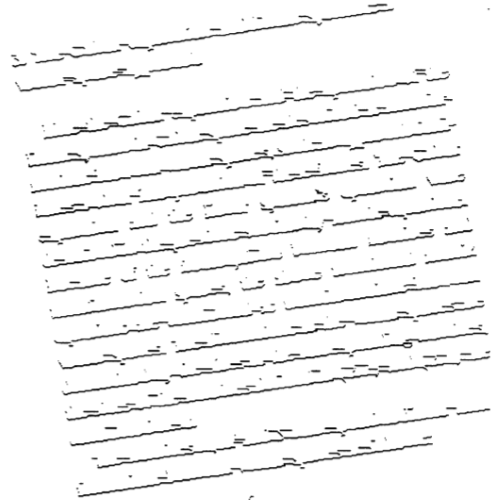
\includegraphics[width=.4\textwidth]{Images/Skew_original.png}
    \captionsetup{justification=centering}
    \caption{Početni nakošeni dokument (slika je preuzeta iz \cite{article:Skew-detection})}
    \label{fig:skew_original}
\end{figure}

Temeljna ideja koja se koristi prilikom izračuna kuta rotacije je ta da se dokument presiječe određenim brojem vertikalnih linija, što je predloženo u radu \cite{article:Skew-detection}.
Za svaku vertikalnu liniju određuju se točke u kojima ona sječe vodoravne linije početnog dokumenta, kao što je prikazano na slici \ref{fig:skew_points}.
Dobivene točke presjecišta označene su kao $T_{n, m}(x_{n, m}, y_{n, m})$, gdje $n$ označava broj vertikalne linije gledano od lijeva na desno, a broj $m$ označava točku presjeka za danu vertikalnu liniju, gledano od gore prema dole.

\begin{figure}[ht!] 
    \centering
    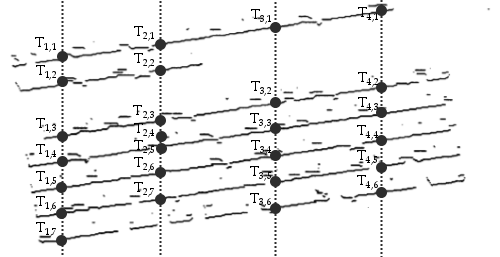
\includegraphics[width=.7\textwidth]{Images/Skew_points.png}
    \captionsetup{justification=centering}
    \caption{Prikaz isječka dokumenta presječenog sa $4$ proizvoljne okomite linije}
    \label{fig:skew_points}
\end{figure}

Jednom kada su određene točke sjecišta, moguće je odabrati jednu takvu točku najljevije vertikalne linije ($T_{1, a}$) te  ju usporediti sa svim točkama linija koje se nalaze desno od nje ($T_{b, c}, \text{t.d. } b \geq 2$).
Dvije tako odabrane točke analiziraju se tako da se kroz njih povuče pravac, čija jednadžba glasi: 
\[
    y - y_{1, a} = k(x - x_{1, a}),
\]
gdje je $k$ koeficijent smjera:
\[
    k = \frac{y_{b, c} - y_{1, a}}{x_{b, c} - x_{1, a}}.
\]
Pomoću koeficijenta  smjera $k$ moguće je izračunati kut pod kojim je dobiveni pravac nagnut u odnosu na $x$ os, kao $\alpha = tan^{-1}(k)$.
Uz pretpostavku da dokument nije rotiran te da se točke $T_{1, a}$ i $T_{b, c}$ nalaze na istim vodoravnim linijama dokumenta, kut $\alpha$ iznosi $0\degree$.
U slučaju da je dokument rotiran, ovako određen kut $\alpha$ bit će jednak stupnju rotacije dokumenta.\\

\begin{figure}[th!]
    \centering
    \begin{subfigure}{.5\textwidth}
        \centering
        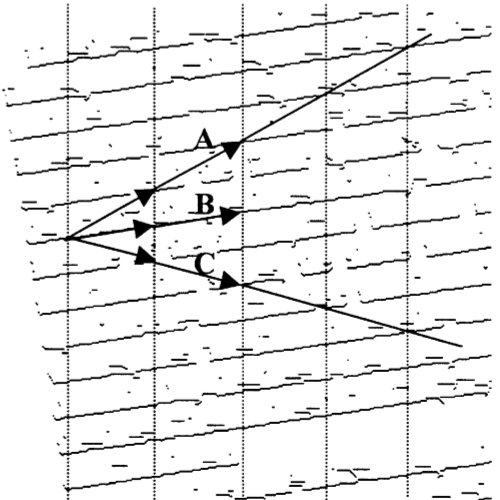
\includegraphics[width=.85\linewidth]{Images/Skew_equidistant.png}
        \captionsetup{justification=centering}
        \caption{Dokument podijeljen ekvidistantnim linijama (slika je preuzeta iz \cite{article:Skew-detection})}
        \label{fig:skew_equidistant}
    \end{subfigure}%
    \begin{subfigure}{.5\textwidth}
        \centering
        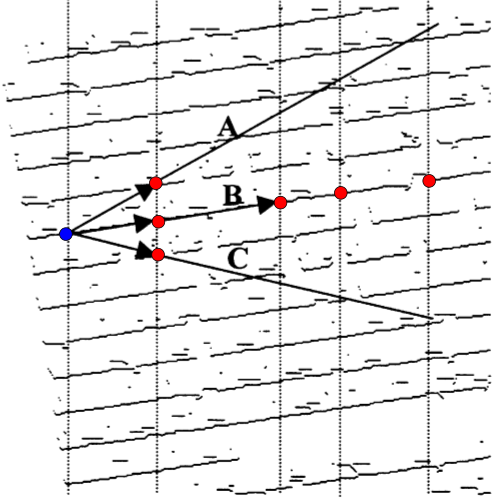
\includegraphics[width=.85\linewidth]{Images/Skew_random.png}
        \captionsetup{justification=centering}
        \caption{Dokument podijeljen linijama sa nasumičnim udaljenostima (slika je preuzeta iz \cite{article:Skew-detection})}
        \label{fig:skwe_random}
    \end{subfigure}
    \caption{Primjer podjele dokumenta okomitim linijama}
    \label{fig:skew_verticalLines}
\end{figure}

Jedan od problema koji preostaje je početna pretpostavka da se točke $T_{1, a}$ i $T_{b, c}$ nalaze na istoj vodoravnoj liniji dokumenta, što neće biti istinito u većini slučajeva.
To se rješava tako da se izračunaju kutevi koje zatvaraju svi pravci koji počinju u točki $T_{1, a}$ i prolaze kroz točku $T_{b, c}$ za svaku moguću točku $T_{b, c}$.
Pritom se bilježi koliko je puta izračunat pojedini kut.
Uz ovaj pristup rotaciju dokumenta više ne određuje kut $\alpha$ koji je dobiven za jedan pravac, već onaj kut koji je najviše puta zabilježen.
Ovaj pristup prikazan je na slici \ref{fig:skew_verticalLines}, gdje je za određenu podjelu vertikalnim linijama i odabranu početnu točku (označeno plavom bojom na slici) prikazan izračun kuteva triju pravaca: \textbf{A}, \textbf{B}, \textbf{C}.
Slika \ref{fig:skew_equidistant} također prikazuje i važnost načina odabira vertikalnih linija kojima se dokument presjeca.
Na navedenoj slici linije su postavljene ekvidistantno, zbog čega dolazi do toga da se sva tri pravca prolaze kroz jednak broj presjecišta horizontalnih i vertikalnih linija.
Posljedica toga je da se svaki od triju prikazanih kuteva javlja $4$ puta što je prikazano crvenim točkama presjecišta, zbog čega nije moguće odrediti koji se kut javlja najveći broj puta.
Za razliku od toga, na slici \ref{fig:skwe_random} koriste se vertikalne linije s nasumičnim međusobnim udaljenostima te se primjećuje kako se na njoj pravac označen sa \textbf{B} prolazi kroz $4$ presjecišta, dok pravci \textbf{A} i \textbf{C} prolaze svaki kroz samo jedno.
Na temelju toga se zaključuje da je kut kojeg pravac \textbf{B} zatvara s $x$ osi jednak rotaciji dokumenta, a da se ostali izračunati kutevi javljaju kao rezultat točaka odabranih na različitim horizontalnim pravcima.

\section{Rezultati}
Kako bi se uštedjelo na vremenu izvođenja, navedeni algoritam je implementiran tako da nakon što odredi nasumične okomite linije odabire samo $4$ početne točke, prethodno označene s $T_{1, a}$.
Za te točke se računaju kutevi sa svim ostalim točkama, a na kraju se provjerava postoji li kut koji prevladava.
Primjer jednog takvog izvođenja prikazan je na slici \ref{fig:skew1}.\\

\begin{figure}[ht!]
    \centering
    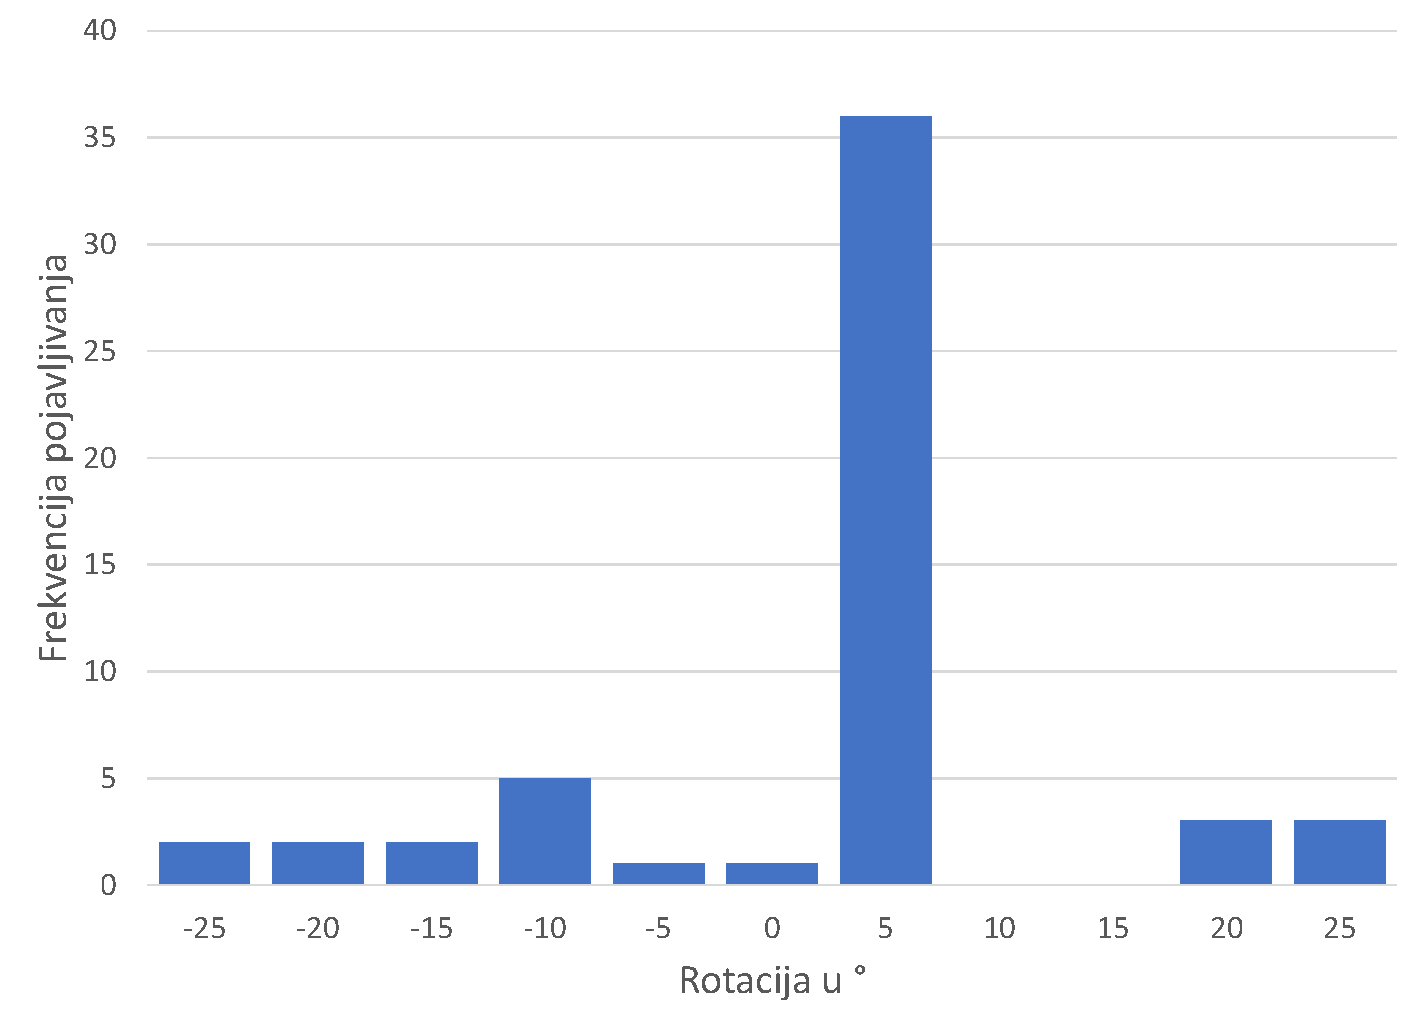
\includegraphics[width=.8\textwidth]{Images/Skew1.pdf}
    \captionsetup{justification=centering}
    \caption{Histogram s prikazom frekvencija pojavljivanja kuteva uz kvant od $5\degree$}
    \label{fig:skew1}
\end{figure}

Iz slike se primjećuje kako je najčešće izmjeren kut od $5\degree$ stupnjeva, iz čega se zaključuje da je slika rotirana za točno taj iznos.
Isti postupak ponovljen je za sliku koja je bila rotirana za kut od $10\degree$ stupnjeva, a rezultati toga prikazani su histogramom na slici \ref{fig:skew2}.
Na ovoj slici se primjećuje kako se za veće iznose kuteva javlja veći šum u izračunatim kutevima, no i dalje je moguće razaznati dominantnu vrijednost kuta rotacije.\\

\begin{figure}[ht!]
    \centering
    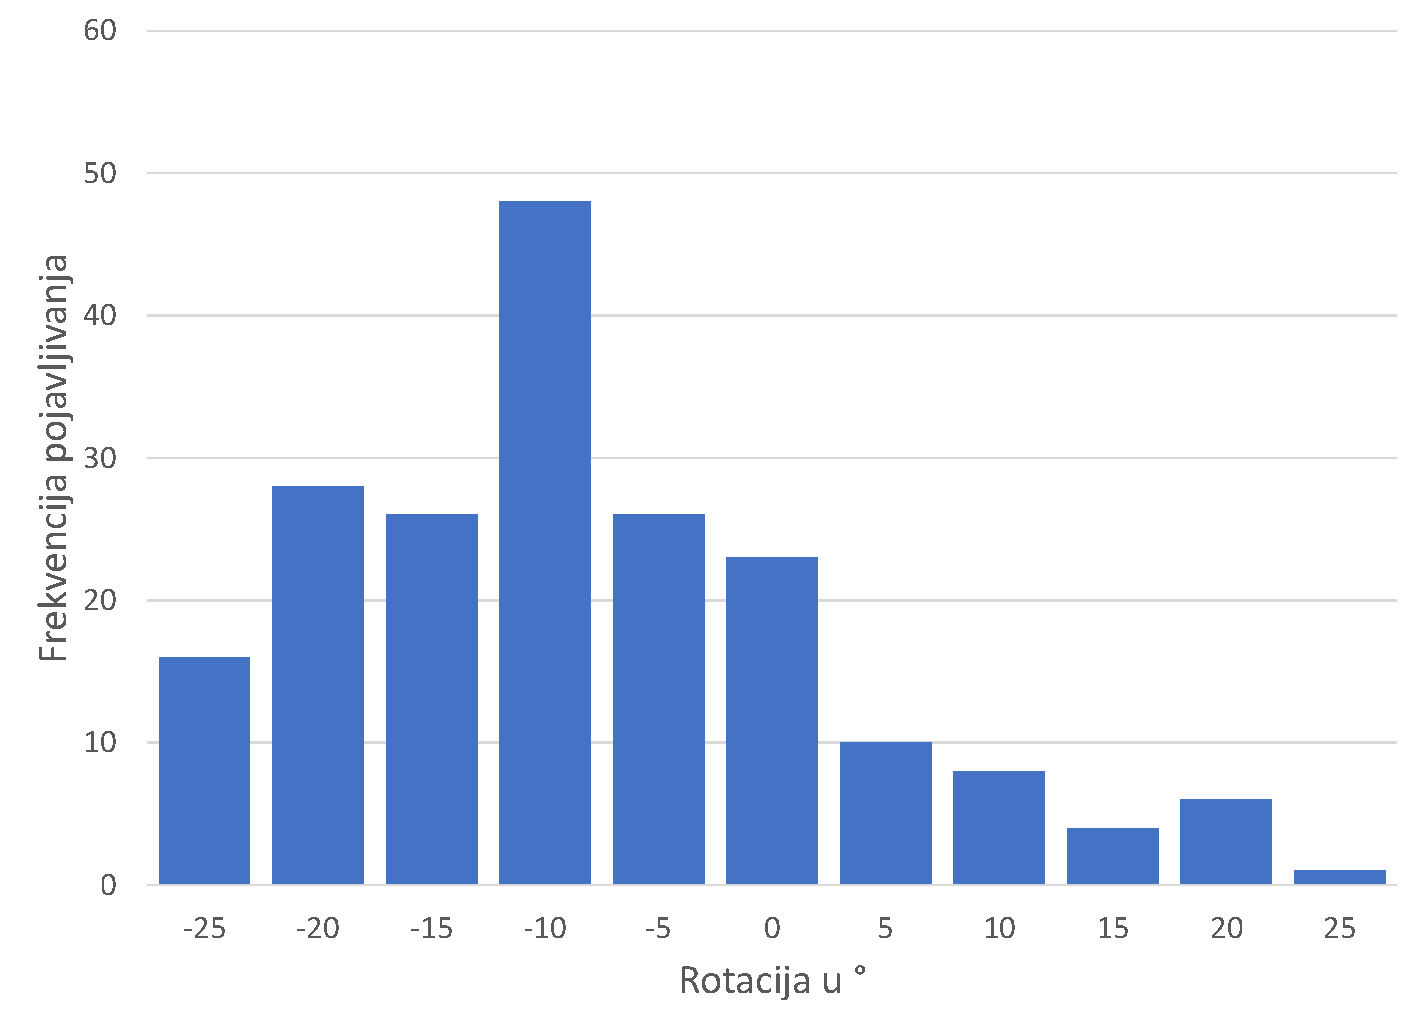
\includegraphics[width=.8\textwidth]{Images/Skew2.pdf}
    \captionsetup{justification=centering}
    \caption{Histogram s prikazom frekvencija pojavljivanja kuteva uz kvant od $5\degree$}
    \label{fig:skew2}
\end{figure}

Problem se javlja kod izračuna koji je prikazan histogramom na slici \ref{fig:skew3}, gdje nije moguće sa sigurnošću odrediti kako je slika rotirana.
Do ovog problema je moglo doći iz više razloga, poput loše odabranih okomitih linija, ili problema zbog točaka dobivenih kao sjecišta okomitih linija i teksta koji se nalazi u tablicama.
Jednostavno i efikasno rješenje navedenog problema je ponovno određivanje okomitih linija te ponovan izračun kuteva s $4$ nove proizvoljne točke.

\begin{figure}[ht!]
    \centering
    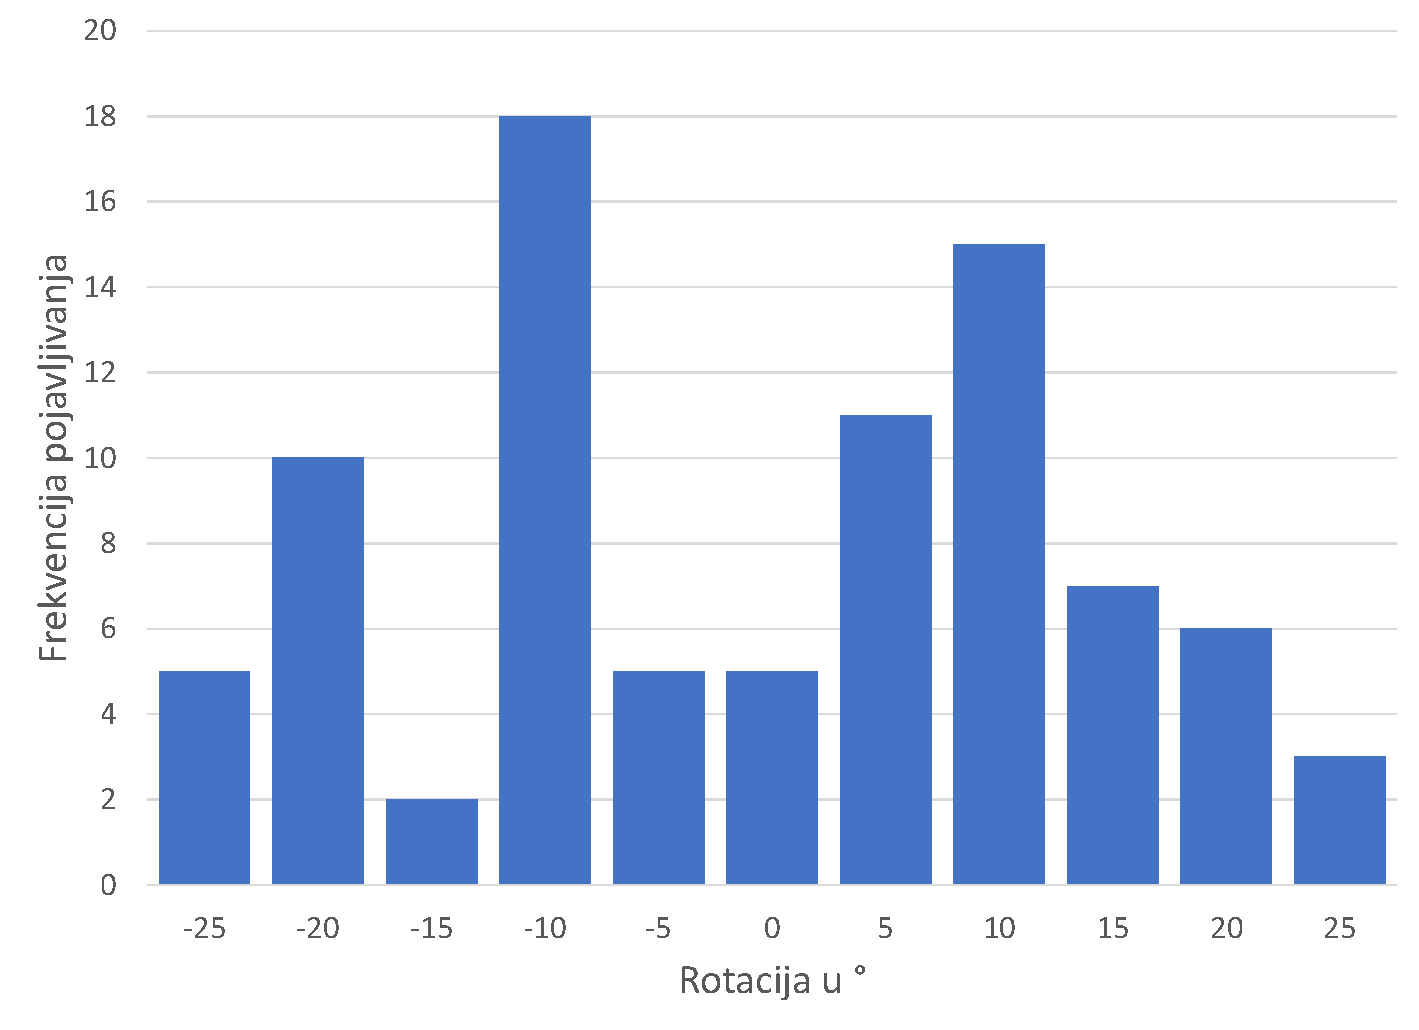
\includegraphics[width=.8\textwidth]{Images/Skew3.pdf}
    \captionsetup{justification=centering}
    \caption{Histogram s prikazom frekvencija pojavljivanja kuteva uz kvant od $5\degree$}
    \label{fig:skew3}
\end{figure}

Opisani postupak korišten je prije daljnje pretrage svih slika opisanih u nastavku rada.

\chapter{Detekcija tablice}
\label{ch:tableDetection}
Kao što je predloženo u radu \cite{conference:AutomaticTableDetectionInDocumentImages}, detekcija tablice temelji se na detekciji vrhova ćelija. 
Analiziranjem općenitih tablica, moguće je uočiti kako postoji $9$ različitih mogućnosti koje se mogu pojaviti kao vrh ćelije, što je prikazano na slici \ref{fig:corners}.

\begin{figure}[ht!]
    \centering
    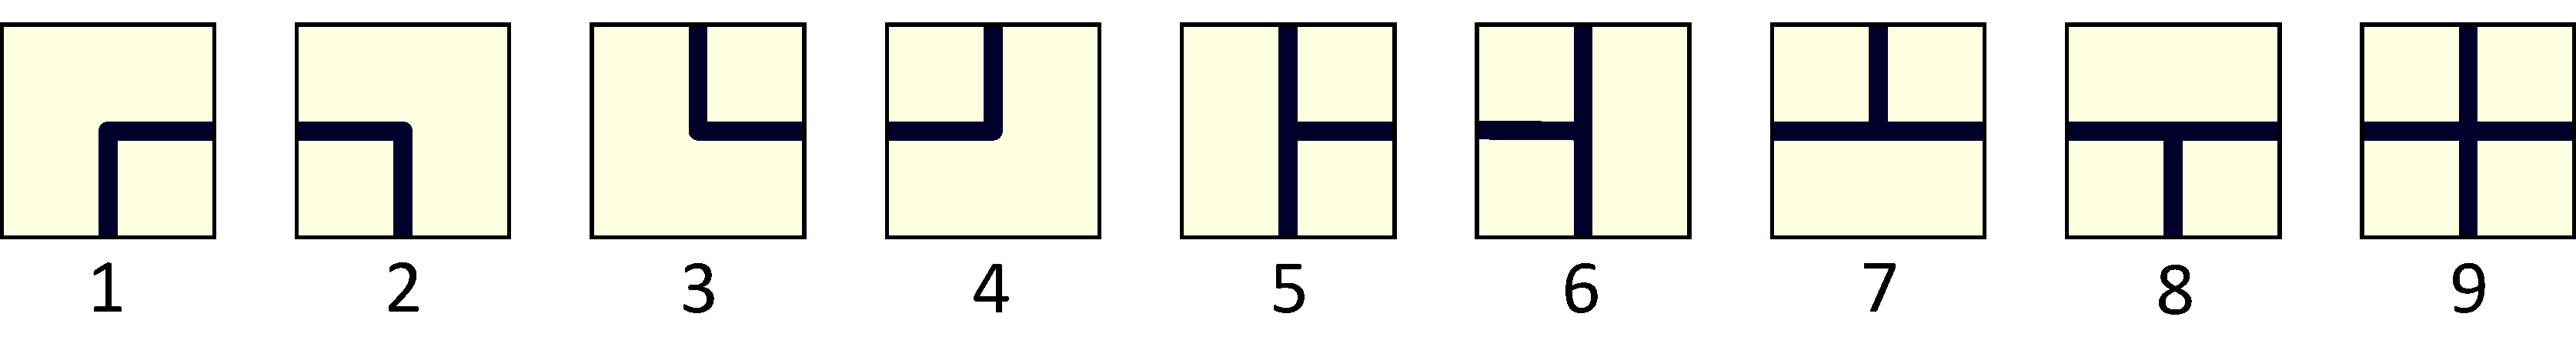
\includegraphics[width=1.0\textwidth]{Images/Corners.pdf}
    \captionsetup{justification=centering}
    \caption{Prikaz mogućih vrsta vrhova ćelija}
    \label{fig:corners}
\end{figure}

Prve $4$ mogućnosti sa slike predstavljaju vrhove ćelija koje su ujedno i vrhovi cijele tablice. 
Sljedeće $4$ mogućnosti izgleda vrha ćelija predstavljaju rubove tablice, odnosno početak ili kraj linija tablice.
Zadnja prikazana mogućnost predstavlja sjecišta linija koja se nalaze unutar tablice.
Detektiranjem točnih pozicija ovih $9$ elemenata te točnom klasifikacijom istih, moguće je jednoznačno rekonstruirati tablicu.\\

Pretragu je moguće ubrzati korištenjem znanja o općem izgledu tablice.
U skladu s time je moguće pronaći isključivo pozicije prve $4$ vrste vrhova, na temelju čega se određuju rubovi tablice.
Koristeći te informacije moguće je odrediti vanjski obrub tablice, na kojemu se moraju nalaziti svi oblici označeni s $5-8$ na slici \ref{fig:corners}, te nije potrebno pretraživati ostatak slike i vršiti klasifikaciju pronađenih kandidata.
Nakon što se pronađu tako opisani rubovi, vrh označen brojem $9$ na slici može se locirati kao sjecište linija između prethodno definiranih rubova tablice.
Ovaj pristup nije detaljnije razrađen u ovom radu te nije korišten u implementaciji, a navodi se isključivo kao prijedlog potencijalne optimizacije korištenog algoritma.

\section{Detekcija vrhova ćelija}
Detekcija vrhova ćelija obavlja se tako da se svaki dio slike provjerava te se za njega utvrđuje prikazuje li on vrh ćelije ili ne. 
Kako bi se to izvelo, potrebno je odrediti točno koji dio slike se provjerava u nekom određenom trenutku, a što se čini korištenjem kliznog prozora. 
Definiran je prozor određenih dimenzija $X$x$Y$ te se promatra samo dio slike unutar njega. 
Tako dobiven isječak slike potom se analizira i ispituje sadrži li on vrh ćelije ili ne.
Jednom kad je detekcija završena za trenutni prozor, prozor se pomiče po $x$ osi za udaljenost $dx$, te se detekcija vrši na tako dobivenom novom isječku slike.
Jedno od mogućih poboljšanja ove metode predloženo je u radu \cite{ViolaJones}, gdje se ne koristi fiksna veličina pomičnog prozora, već se pretraga započinje s jednom veličinom prozora te se ona iterativno smanjuje tijekom pretrage.


\subsection{Određivanje značajki}
Prije nego li se može napraviti detekcija vrhova, potrebno je definirati značajke prema kojima se isti pretražuju.
Osnovna funkcija značajki je pojednostavljenje slike koja se pokušava prepoznati kako bi se smanjio ukupan prostor pretraživanja.
Potrebno je odrediti značajke koje vrijede neovisno o manjim pomacima slike, ili manjim šumovima koji mogu biti prisutni iz različitih razloga.
Za potrebe toga odabrana su dva različita pristupa odabira značajki.\\

Prvi korišteni način zasniva se na činjenici da se detektiraju dijelovi tablica, koje se sastoje isključivo od vodoravnih i okomitih linija.
Imajući to na umu moguće je uočiti da će u idealnom slučaju okomite i vodoravne zrake (prikazano crvenom bojom) sjeći vrh ćelije uvijek u samo jednoj točki, kao što je prikazano u primjeru na slici \ref{fig:lineFeatures}.

\begin{figure}[th!]
    \centering
    \begin{subfigure}{.5\textwidth}
        \centering
        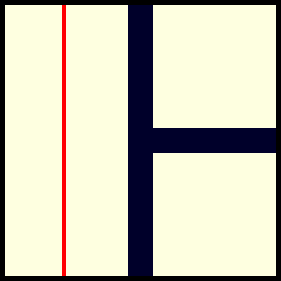
\includegraphics[width=.3\linewidth]{Images/LineFeature.pdf}
        \captionsetup{justification=centering}
        \caption{Primjer zrake bez sjecišta}
        \label{fig:feature1}
    \end{subfigure}%
    \begin{subfigure}{.5\textwidth}
        \centering
        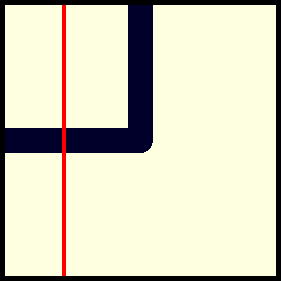
\includegraphics[width=.3\linewidth]{Images/LineFeature1.pdf}
        \captionsetup{justification=centering}
        \caption{Primjer zrake sa sjecištem}
        \label{fig:feature2}
    \end{subfigure}
    \caption{Primjer ekstrakcije značajki korištenjem okomite zrake}
    \label{fig:lineFeatures}
\end{figure}

Ovisno o koordinati zrake moguće je odrediti koja je to vrsta vrha, točnije na danom primjeru na slici \ref{fig:feature1} nema sjecišta zrake i linije, iz čega se zaključuje kako se na slici ne nalaze određeni vrhovi ćelija, poput, na primjer, vrha označenog brojem $2$ na slici \ref{fig:corners}, koji ima vodoravnu liniju na lijevoj strani.
Ista ta zraka na primjeru na slici \ref{fig:feature2} presijeca sliku na jednom mjestu, iz čega se zaključuje da se na slici potencijalno nalazi vrh koji na tom mjestu ima liniju.\\

Ovaj pristup se nadopunjuje tako da se umjesto broja presjecišta određuje udaljenost od prvog presjecišta.
Na taj se način razlikuje linija koja se očekivano pojavljuje na sredini slike od šuma koji se može pojaviti na svim mjestima slike.
Prilikom ovog pristupa koji uključuje izračun udaljenosti do presjecišta potrebno je relativizirati dobivenu udaljenost u odnosu na veličinu slike na kojoj se radi analiza kako bi se osiguralo da značajke ne ovise o veličini slike.
Osim navedenoga, koriste se i dijagonalne zrake s kojima se određuje broj presjecišta kako bi se dodatno povećala raznolikost značajki, a samim time i robusnost algoritma.\\

Drugi pristup određivanja značajki slike temelji se na pristupu koji je korišten u radu \cite{ViolaJones}.
Ove značajke temelje se na činjenici da različiti dijelovi slike sadrže različitu količinu crnih slikovnih elemenata.
Kao što je prikazano na slici \ref{fig:haarFeatures}, gdje su prikazana $4$ različita oblika značajki ovog tipa koje se koriste u ovome radu, značajke se računaju za određeni dio slike, što je prikazano pravokutnikom.
Vrijednost značajke se računa kao razlika broja crnih slikovnih elemenata u crnom i bijelom djelu pravokutnika.
Kako bi se postigla neovisnost o veličini slike nad kojom se vade značajke, izračunata razlika broja slikovnih elemenata dijeli se ukupnim brojem slikovnih elemenata u kvadratu značajke.
Na ovaj način se ispituje je li neko područje tamnije od njemu susjednog područja, što je primjer kod linija tablice, gdje se linija nalazi na sredini promatranog područja koje je zbog toga tamno, a neposredno pored nje se nalazi bijelo područje. 
Potencijalne smetnje koje mogu nastati na slici kao posljedica sadržaja tablice ne utječu značajno na vrijednost značajke, budući da značajka obuhvaća veću površinu, a potencijalne smetnje se u većini slučajeva nalaze na manjem lokalnom području.

\begin{figure}[th!]
    \centering
    \begin{subfigure}{.25\textwidth}
        \centering
        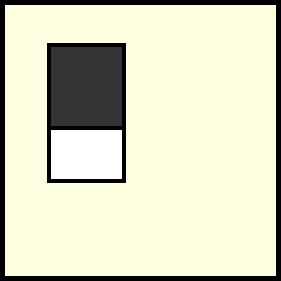
\includegraphics[width=.5\linewidth]{Images/Haar_VD.pdf}
        \captionsetup{justification=centering}
        \caption{}
        \label{fig:haar1}
    \end{subfigure}%
    \begin{subfigure}{.25\textwidth}
        \centering
        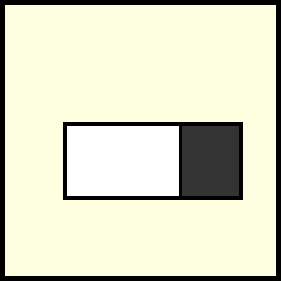
\includegraphics[width=.5\linewidth]{Images/Haar_HD.pdf}
        \captionsetup{justification=centering}
        \caption{}
        \label{fig:haar2}
    \end{subfigure}%
    \begin{subfigure}{.25\textwidth}
        \centering
        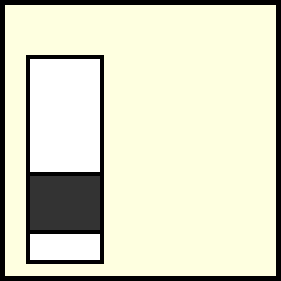
\includegraphics[width=.5\linewidth]{Images/Haar_VT.pdf}
        \captionsetup{justification=centering}
        \caption{}
        \label{fig:haar3}
    \end{subfigure}%
    \begin{subfigure}{.25\textwidth}
        \centering
        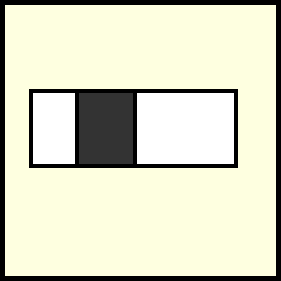
\includegraphics[width=.5\linewidth]{Images/Haar_HT.pdf}
        \captionsetup{justification=centering}
        \caption{}
        \label{fig:haar4}
    \end{subfigure}
    \caption{Primjeri značajki temeljenih na razlici količine boje}
    \label{fig:haarFeatures}
\end{figure}

Prednost ovog skupa značajki je mogućnost izračuna istih u konstantnoj složenosti, uz prethodno pretprocesiranje podataka.
Računa se novi oblik reprezentacije slike ($ii$) u kojemu je vrijednost na poziciji $x, y$ jednaka ukupnom broju crnih slikovnih elemenata na početnoj slici za sve elemente koji se nalaze gore lijevo od trenutnog, odnosno:
\[
    ii(x, y) = 
        \displaystyle \sum_{x' < x} 
        \displaystyle \sum_{y' < y}
        i(x', y').
\]

\begin{figure}[ht!]
    \centering
    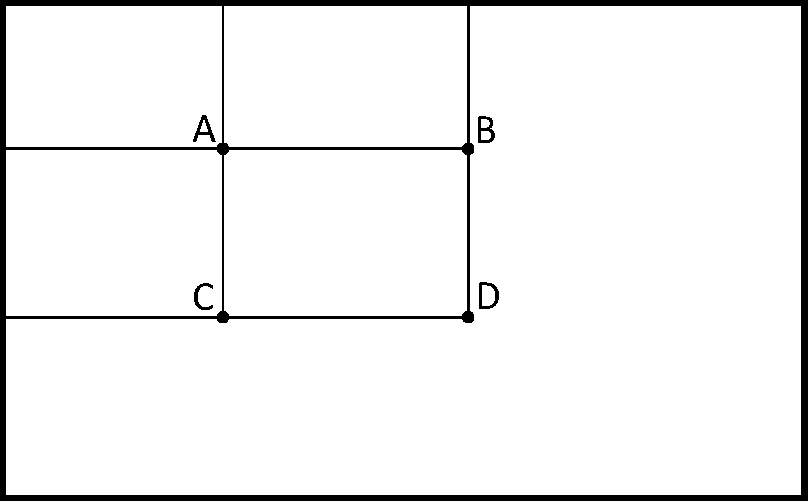
\includegraphics[width=0.5\textwidth]{Images/Integral.pdf}
    \captionsetup{justification=centering}
    \caption{Primjer izračuna broja crnih elemenata unutar kvadrata}
    \label{fig:integral}
\end{figure}

Ove vrijednosti je moguće izračunati jednim prolazom kroz početnu sliku. 
Korištenjem ovih suma moguće je izračunati broj crnih elemenata za bilo koji kvadrat na početnoj slici.
Primjer izračuna prikazan je slikom \ref{fig:integral}, na kojoj je prikazan kvadrat $ABCD$ za kojega želimo izračunati opisanu vrijednost. 
Važno je uočiti da su prethodno već izračunate sume od gornjeg lijevog kuta do svake pojedine točke.
Traženu vrijednost je moguće prikazati kao kumulativnu sumu u točki $D$, što uključuje cijeli kvadrat, kao i područja lijevo i iznad njega.
Vrijednost područja koje se nalazi lijevo od kvadrata jednaka je sumi u točki $C$ te se ta vrijednost oduzima od prethodne vrijednosti.
Analogno tome, od trenutne vrijednosti oduzima se suma u točki $B$.
Trenutni postupak je u dva navrata oduzeo vrijednost područja koje se nalazi gore lijevo od točke $A$ pravokutnika, zbog čega je potrebno trenutnoj vrijednosti jednom pridodati sumu u točki $A$.
Konačna vrijednost za dani kvadrat glasi:
\[
    f = ii(D_x, D_y) - ii(C_x, C_y) - ii(B_x, B_y) + ii(A_x, A_y).
\]

\subsection{Detekcija korištenjem umjetne neuronske mreže}
Umjetne neuronske mreže nastale su kao model kojim se nastoji simulirati način rada ljudskog mozga.
U nastavku je ukratko opisan način rada istih, dok se detaljnije objašnjenje može pronaći u knjizi \cite{umjetnaInteligencija}.
Poznato je da se mozak sastoji od velikog broja međusobno povezanih neurona.
Svaki se neuron sastoji od $3$ djela: dendrita koji primaju električne podražaje, tijela koje reagira na podražaj i aksona koji prosljeđuje podražaj sljedećim povezanim neuronima.
Osnovni princip rada neurona temelji se upravo na spomenutoj propagaciji električnih impulsa. 
Umjetni neuroni simuliraju pojednostavljeni model bioloških neurona tako da oponašaju prethodno navedene funkcionalnosti.

\begin{figure}[ht!]
    \centering
    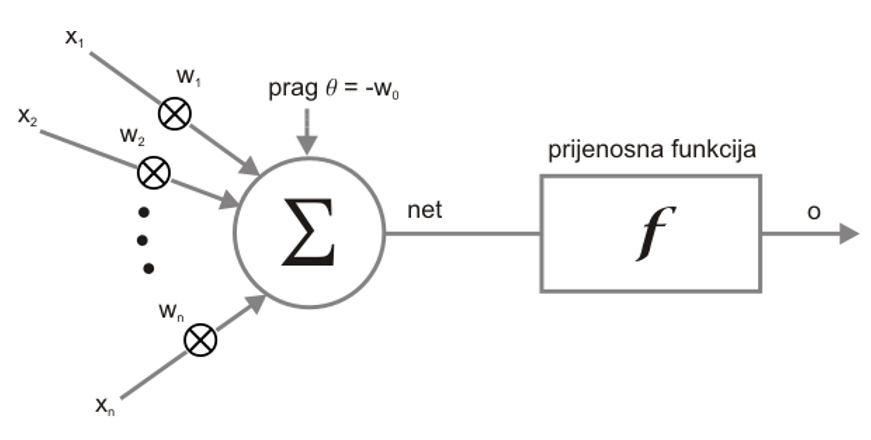
\includegraphics[width=0.5\textwidth]{Images/Neuron.png}
    \captionsetup{justification=centering}
    \caption{Prikaz modela umjetnog neurona}
    \label{fig:neuron}
\end{figure}

Slika \ref{fig:neuron} prikazuje opći model takvog neurona. 
Ulazne vrijednosti neuronu čine vrijednosti od $x_1$ do $x_n$, te se svakoj od njih dodjeljuje određena težina $w_1$ do $w_n$ s kojom se ulazna vrijednost množi.
Na taj se način ostvaruje mogućnost postavljanja različitih prioriteta različitim ulazima.
Tijelo neurona ostvareno je funkcijom sumacije koja zbraja težinske vrijednosti ulaza i praga te tako dobiveni broj predaje prijenosnoj funkciji, koja se ponaša kao model aksona.
Prijenosna funkcija za dani argument vraća rezultat iz određenog raspona, što se propagira kao ulaz sljedećim neuronima.\\

Korištenjem samo jednog neurona moguće je ostvariti jednostavnije linearne klasifikacijske algoritme, tako da se kao ulazi neurona koriste značajke prema kojima se klasificira, a za prijenosnu funkciju odabere funkcija skoka.
Ovisno o izlazu iz neurona uzorak se klasificira u jedan od dva razreda.
Prvi nedostatak ovog modela koji se uočava je nemogućnost istoga da uzorak klasificira ako postoji više različitih razreda.
Taj se problem može riješiti dodavanjem novih neurona koji primaju jednake ulaze kao i prvi neuron, te izlaz svakog od njih odgovara pojedinom razredu u koji ulazni uzorak može biti klasificiran.
Takva grupacija neurona zove se sloj neuronske mreže.\\

Sljedeći problem dobivenog modela je mogućnost rada isključivo s linearno odvojivim podatcima. 
Taj se problem rješava dodavanjem novih slojeva neurona u neuronsku mrežu, tako da se izlazi neurona jednog sloja proslijede kao ulazi neuronima drugog sloja.
Pri tome se razlikuju $3$ općenite vrste slojeva: ulazni sloj neurona koji služi kako bi se ulazne vrijednosti značajki proslijedile ostatku neuronske mreže, skriveni sloj neurona koji se koristi prilikom računanja, ali nije vidljiv vanjskom korisniku te izlazni sloj, čiji se rezultat predaje krajnjem korisniku.

\begin{figure}[ht!]
    \centering
    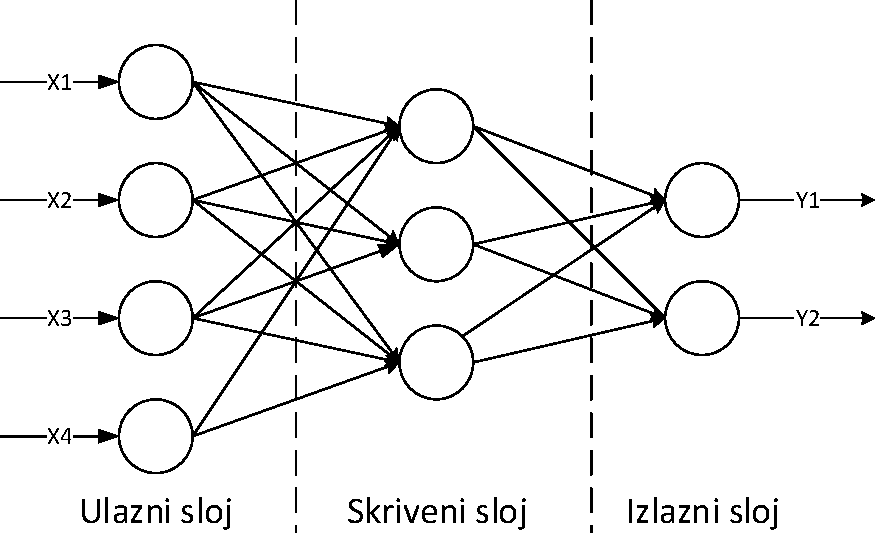
\includegraphics[width=0.7\textwidth]{Images/FFANN.pdf}
    \captionsetup{justification=centering}
    \caption{Model unaprijedne neuronske mreže}
    \label{fig:ffann}
\end{figure}

Ovisno o načinu povezivanja neurona moguće je ostvariti različite arhitekture umjetnih neuronskih mreža. 
U radu je korištena unaprijedna neuronska mreža, kakva je prikazana na slici \ref{fig:ffann}.
Jedna od prednosti umjetnih neuronskih mreža leži u mogućnosti učenja istih, a što je moguće učiniti promjenom težina ulaza za pojedini neuron.
Jednom kad je mreža naučena, odnosno kada su određene težine uz koje mreža zadovoljavajuće izvršava zadatak za koji je predviđena, dobivene težine pohranjuju se u datoteku na računalu kako se za daljnja pokretanja mreža ne bi morala ponovno učiti.
Ovo svojstvo omogućava veliku brzinu klasifikacije jednom kada je mreža naučena.

\subsection{Detekcija algoritmom AdaBoost}
Umjetne neuronske mreže izvode velik broj računskih operacija kako bi klasificirale neki ulazni primjer.
To predstavlja problem kada je potrebno klasificirati velik broj uzoraka, kao što je to slučaj kod detekcije vrhova ćelija, gdje je potrebno za svaki mogući element slike odrediti je li on vrh ćelije ili ne.
Kako bi se taj postupak ubrzao koristi se drugačiji pristup klasificiranju primjenom bržih algoritama. \\

Osnovna ideja algoritma AdaBoost je izgraditi jedan jaki klasifikator primjenom više slabih klasifikatora.
U okviru ovog algoritma, jaki klasifikator je finalni klasifikator koji uz veliku točnost podatke raspoređuje u jednu od grupa, dok su slabi klasifikatori u stanju točno klasificirati samo manji podskup podataka, dok ostale svrstavaju u krive grupe.\\

Slabi klasifikatori određuju fiksni prag za kojega će nešto klasificirati u jednu ili drugu kategoriju, ovisno o vrijednosti korištene značajke za sliku. Takav klasifikator prikazan je sljedećom funkcijom:
\[
    h(x, f, p, \theta) = 
    \begin{cases}
    1,  & \quad \text{ako je } pf(x) < p\theta \\
    0,  & \quad \text{inače},\\
    \end{cases}
\]
gdje je s $h(x, f, p, \theta)$ označen klasifikator, s $x$ uzorak, s $f$ funkcija koja na temelju uzorka određuje značajku, a $p$ predstavlja faktor koji određuje smjer nejednakosti, ovisno o predznaku.
Ukupna greška ovakvog klasifikatora definirana je kao težinska suma svih odstupanja, gdje se svakom uzorku pridjeljuje određena težina kojom on doprinosi ukupnoj grešci.
Izračun ukupne greške $\epsilon$ prikazan je izrazom:
\[
    \epsilon = \displaystyle \sum_{i}w_i \abs{h(x, f, p, \theta) - y_i}, 
\]
gdje je s $w_i$ predstavljena težina $i$-tog po redu uzorka, a s $y_i$ očekivana vrijednost izlaza klasifikatora.
Ovako definirani klasifikator točno klasificira samo manji podskup podataka.
U postupku učenja istih potrebno je odrediti parametre $x, f, p, \theta$ koji za trenutno postavljene težine $w$ minimiziraju pogrešku $\epsilon$. 
Točan postupak pronalaženja takvog slabog klasifikatora opisan je u poglavlju \ref{ch:implementation} gdje je objašnjena implementacija algoritma.
Prilikom izgradnje jakog klasifikatora koji uz veliku točnost klasificira podatke koriste se ovako dobiveni slabi klasifikatori, ali se pritom svaki sljedeći slabi klasifikator određuje nakon što se težine $w$ promijene, kako bi se postiglo da sljedeći slabi klasifikator veći prioritet daje podatcima koji su prethodno pogrešno klasificirani, točan postupak dan je u nastavku.\\

Jaki klasifikatori grade se kao spoj više slabih klasifikatora tako da se računa izlaz svakog od njih te se na temelju toga donosi konačna odluka o kategoriji u koju treba svrstati ulazni uzorak.
Kako bi se stvorio jaki klasifikator potrebno je odrediti skup labeliranih ulaznih primjera koji se koriste tijekom učenja.
Budući da algoritam može klasificirati samo $2$ kategorije podataka, potrebno mu je predati uzorke koje smije i koje ne smije prepoznati, gdje je s $1$ označen uzorak koji se prepoznaje, a s $0$ uzorak koji se ne prepoznaje.
Na slučaju tablica, algoritam prepoznaje sve oblike vrhova ćelija, a pritom ne prepoznaje sadržaj unutar tablice, linije tablice i ostale smetnje koje se pojavljuju na slici.
Početne težine za svaki od uzoraka postavljene su na: 
\[
    w_i = 
    \begin{cases}
    \frac{1}{m}, & \quad y_i = 0\\
    \frac{1}{l}, & \quad y_i = 1.\\
    \end{cases}
\]
Pritom je s $m$ označen broj negativnih uzoraka, a s $l$ broj pozitivnih uzoraka.
Potom se ovisno o željenom broju slabih klasifikatora ponavlja sljedeći postupak.
Prvo je potrebno normalizirati sve težine:
\[
    w_i \leftarrow \frac{w_i}{
        \displaystyle \sum_{j = 1}^{n}w_j
    }.
\]
Potom se određuje slabi klasifikator $h$ koji za trenutne težine daje najmanju pogrešku $\epsilon$, izračunatu na prethodno opisani način.
Dobiveni slabi klasifikator ne može točno klasificirati određeni dio podataka, zbog čega je potrebno postići da sljedeći slabi klasifikator uspješno prepozna te podatke.
To se postiže mijenjanjem trenutnih težina korištenih u izračunu greške tako da se povećavaju težine onih ulaza čija je vrijednost pogrešno klasificirana, a smanjuju težine ulaza čija je vrijednost ispravno klasificirana, prema formuli:
\[
    w_i \leftarrow 
    \begin{cases}
        w_i\beta, & \quad \text{ako je uzorak $i$ točno klasificiran}\\
        w_i, & \quad \text{inače.}\\
    \end{cases}
\]
Pritom je koeficijent $\beta$ definiran kao: 
\[
    \beta = \frac{\epsilon}{1 - \epsilon}.
\]
Za ovako određen slabi klasifikator računa se još i vrijednost $\alpha$ kao: 
\[
    \alpha = log(\frac{1}{\beta}),
\]
što se koristi prilikom izrade konačnog jakog klasifikatora tako da izlazi klasifikatora s većom vrijednošću $\alpha$ više doprinose konačnoj odluci klasifikacije od onih s manjom vrijednošću.
Jaki klasifikator određen je kao:
\[
    C(x) = 
    \begin{cases}
        1, & \quad 
            \displaystyle \sum_{t = 1}^{T}
            \alpha_th_t(x)
            \geq
            \frac{1}{2} \displaystyle \sum_{t = 1}^{T}\alpha_t\\
        0, & \quad \text{inače.}\\
    \end{cases}
\]

Prednost ovako dobivenog klasifikatora leži u njegovoj brzini, pogotovo ako se kao značajke na temelju kojih se vrši klasifikacija koriste značajke koje je moguće jednostavno izračunati, poput druge skupine značajki opisanih u ovome radu.


\subsection{Kombiniranje klasifikatora}
Prethodno su objašnjena dva različita klasifikatora korištena prilikom detekcije tablica.
Svaki od njih ima svoje prednosti, ali i mane.
Kako bi se iskoristile dobre strane svakoga od njih, moguće je napraviti novi klasifikator koji će raditi korištenjem prethodno opisana dva klasifikatora.
Za potrebe toga korišten je jaki klasifikator nastao korištenjem algoritma AdaBoost koji analizira cijelu sliku te određuje točke od potencijalnog interesa. 
To su točke na kojima je klasifikator rekao da se nalaze vrhovi ćelija, ali zbog prirode klasifikatora nije moguće znati točno o kojim je vrhovima riječ.
Također, nije nužno potrebno da ovaj klasifikator izbaci sve točke koje ne sadrže vrhove tablica, jer se sve pronađene točke ponovno klasificiraju korištenjem umjetne neuronske mreže.\\

Umjetna neuronska mreža koristi se kako bi se za prethodno dobivene točke interesa odredilo koju vrstu vrha ćelije predstavljaju.
Za potrebe toga moguće je koristiti neuronsku mrežu koja radi s većim brojem ulaznih značajki, bez opasnosti od velikog vremena izvođenja, zahvaljujući činjenici da se neuronska mreža pokreće na malom skupu točaka slike. 

\section{Rekonstrukcija tablice}
Korištenjem prethodno opisanih klasifikatora dobiven je popis vrhova ćelija tablice s prepoznatom vrstom vrha i koordinatom na kojoj se nalazi.
Potrebno je na temelju tog znanja odrediti točan izgled tablice. 
Poznavanjem pozicija vrhova označenih s $1, 2, 3$ i $4$ na slici \ref{fig:corners} određena je točna lokacija tablice. 
Ovisno o broju vrhova ovog tipa moguće je odrediti i točan izgled tablice u slučaju da ona nije pravilnog kvadratnog oblika.
Vrhovi označeni s $5, 6, 7$ i $8$ određuju vanjski obrub tablice, dok je unutrašnjost iste određena vrhovima tipa $9$ sa slike \ref{fig:corners}.
Kako bi se ćelije točno poredale u prostoru potrebno je sortirati popis vrhova istih po jednoj, pa zatim po drugoj koordinati.
Tako je moguće vrhove rasporediti u dvodimenzionalno polje na način da se svi vrhovi s približno jednakom vrijednošću $Y$-koordinate, uz pretpostavku da je slika izravnata postupkom opisanom u poglavlju \ref{ch:skewDetection}, pohrane u isti red polja, te tako definiraju isti redak tablice.
Ponavljanjem postupka za sve različite vrijednosti $Y$ koordinata određuju se svi redci, a kako su točke prethodno bile sortirane vrijedi da $n$-ta točka svakog retka opisuje $n$-ti stupac tablice.

\section{Korištenje prethodno stečenog znanja}
Prilikom prvog prepoznavanja tablice nije moguće pretpostaviti ništa o njezinom izgledu te je do sada opisana metoda jedina točna i efikasna mogućnost.
Kada se prepoznaje veći broj tablica koje su strukturno jednake te se nalaze na istim pozicijama na papiru, moguće je ubrzati pretragu tablica korištenjem znanja stečenog prilikom detekcije prve tablice. 
Zbog mogućnosti pomaka papira u postupku digitalizacije nije moguće očekivati da se vrhovi ćelija nalaze na točno jednakim pozicijama na slici dokumenta.
Zbog toga je potrebno izvršiti ponovnu pretragu slike kako bi se odredile nove pozicije.
Primjećuje se kako nije potrebno ponovno pretražiti područje cijele slike, već se pretražuju samo područje unutar zadanog radijusa oko pozicija vrhova s prethodno prepoznate tablice.\\

Opisani postupak moguće je dodatno ubrzati tako da se ne pretražuju ponovno svi vrhovi tablice, već samo jedan, poput na primjer gornjeg lijevog vrha.
Nakon što se pronađe točna pozicija tog vrha na novoj slici zaključuje se kako je cijela tablica, odnosno svi vrhovi njezinih ćelija, pomaknuta za isti iznos u odnosu na prvotno detektiranu kao i pronađeni vrh.
Mana ovog pristupa je velika osjetljivost na rotacije i ostale moguće pomake papira u postupku digitalizacije. 
Problem rotacije je djelomično riješen prethodno opisanim postupkom detekcije zakrivljenosti slike, no unatoč tome postoji mogućnost da slika i nakon ispravka rotacije ostane blago rotirana, što za tablice većih dimenzija može predstavljati problem.
Zbog opisanih problema ovaj je pristup odbačen te je korišten sporiji postupak opisan u prethodnom odlomku.


\chapter{Implementacija i rezultati} 
\label{ch:implementation}
Svi postupci opisani u ovom radu implementirani su u programskom jeziku Java.
Izvorni kodovi su javno dostupni su na adresi \href{https://github.com/vkristijan/Table-Extraction-on-Scanned-Documents}{https://github.com/vkristijan/Table-Extraction-on-Scanned-Documents}.

\section{Umjetna neuronska mreža}
Kao što je prethodno opisano, prilikom klasifikacije se koristi unaprijedna umjetna neuronska mreža. 
Mreža koristi arhitekturu sa $3$ sloja.
Prvi, odnosno ulazni sloj sadrži $24$ neurona, koji kao ulaz primaju vrijednosti $24$ različite značajke.
Skriveni sloj sadrži $14$ neurona, a izlazni $10$.\\

Kao značajke koje se koriste kao ulaz koriste se ručno odabrane značajke. 
Imajući na umu izgled slika koje je potrebno klasificirati, uočava se kako su slike pravilne i međusobno simetrične, zbog toga će u daljnjem tekstu biti navedene samo značajke koje koriste okomite zrake, odnosno okomite kvadrate prebrojavanja slikovnih elemenata, premda se u stvarnosti koriste jednake takve značajke i za vodoravne zrake odnosno kvadrate prebrojavanja slikovnih elemenata.\\

Prvo što je potrebno uočiti je da se kod svih objekata koje je potrebno prepoznati linije nalaze na sredini slike.
Ako slika koja se klasificira sadrži liniju koja se nalazi na nekoj drugoj poziciji, primjerice vodoravna linija na samom vrhu slike, tada na slici nije prikazan vrh ćelije, odnosno ako i je prikazan, tada točka vrha nije približno u središtu slike.
Kako bi se to provjerilo, dodane su dvije značajke koje određuju udaljenost do najbližeg crnog slikovnog elementa, jedna od njih gleda udaljenosti po okomitoj zraci koja se nalazi na udaljenosti $0.1$ od ukupne širine slike, a druga na udaljenosti $0.9$.
Svaka od tih značajki generira dvije vrijednosti, udaljenost od gornjeg ruba slike do prvog crnog elementa te udaljenost od donje linije do prvog crnog elementa.
Ove značajke vraćaju kvalitetnu informaciju o tome gdje se na slici nalazi linija, ali nisu otporne na potencijalne smetnje na slici.
Kao rješenje tog problema koriste se značajke dobivene kao broj sjecišta s okomitim zrakama, na udaljenosti $0.25$, odnosno $0.35$ širine slike od lijevog, odnosno desnog ruba.
Tako dobivene $4$ značajke su u stanju kvalitetno prikazati postoji li linija na tom mjestu ili ne, ali ne provjeravaju položaj linije, što je napravljeno prethodnim značajkama.
Kako bi se omogućila dodatna robusnost algoritma, primijenjene su značajke koje su prikupljene kao broj presjecišta korištenjem dijagonalnih zraka.
Kako vrh ćelije nije uvijek nužno u središtu slike moguće je da zraka koja prolazi dijagonalom ne prolazi vrhom te zbog toga ima $2$ sjecišta umjesto jednoga.
Taj je problem riješen odmicanjem dijagonalnih zraka od glavne dijagonalne za određenu konstantnu vrijednost, čime se može provjeriti postoje li dvije okomite linije u određenom kvadrantu slike, ako postoje $2$ sjecišta.
Ovisno o odmaku od središnje dijagonale ovisi i tolerancije prema odmaku središta vrha ćelije u odnosu na središte linije.
Uz navedene, koriste se značajke koje se temelje na razlici broja crnih slikovnih elemenata u određenim kvadratnim područjima.
Za potrebe toga definirana su $2$ značajke koje prikupljaju informacije o postojanju vodoravne linije. 
Obje značajke koriste pravokutnik za uzorkovanje kakav je prikazan na slici \ref{fig:haar3}, a pravokutnici se po širini protežu od $0.1$ do $0.9$ širine slike uzorka.
Visine pravokutnika se razlikuju te jedan prekriva većinu visine slike, dok je crno područje definirano kao uži dio oko centra slike.
Tako ova značajka pruža uvid u odnos cjelokupne slike, ali zbog toga na nju jače utječu ostali crni elementi prisutni na slici.
Kao rješenje tog problema koristi se drugi pravokutnik koji ima manju visinu zbog čega manje ovisi o ostatku slike, a više o prisutnosti linije.

\subsection{Treniranje genetskim algoritmom}
Prvi pokušaj treniranja neuronske mreže bio je korištenjem genetskog algoritma, koji su opisani u knjigama \cite{optjava} i \cite{GeneticAlgorithms}.
Genetski algoritmi jedan su od često korištenih metaheurističkih algoritama.
Nastali su po uzoru na Darwinovu teoriju evolucije, koja se temelji na sljedećih pet pretpostavki: 
\begin{enumerate}
\item uvijek postoji više potomaka nego što je potrebno
\item veličina populacije je približno stalna
\item količina hrane je ograničena
\item razmnožavanjem jedinki nastaju nove, različite jedinke
\item većina varijacija prenosi se nasljeđivanjem.
\end{enumerate}
Iz navedenih pretpostavki slijedi da ne mogu preživjeti sve jedinke zbog limitiranih resursa.
Zbog toga dolazi do pojave da neke jedinke umiru, a preživljavaju one prilagođenije.
Tako s vremenom ukupna populacija postaje prilagođenija okruženju u kojemu se nalazi.\\

Genetski algoritmi modeliraju uočeno ponašanje iz prirode tako da rješenje problema prikazuju kao kromosom koji definira jednu jedinku.
Za svaku jedinku moguće je odrediti funkciju njezine dobrote, koja predstavlja uspješnost te jedinke, pri čemu je cilj da uspješnije jedinke preživljavaju kako bi ukupna populacija težila optimalnom rješenju.
Korištenjem operatora križanja moguće je iz dvije jedinke stvoriti novu, pri čemu se dio kromosoma jedne jedinke te dio kromosoma druge jedinke prenosi na novonastalu jedinku.
Nad novodobivenom jedinkom se tada primjenjuje operator mutacije čime se uvodi novi genetski materijal u populaciju i nastoje izbjeći lokalni optimumi.
Primjer rada takvog algoritma prikazan je slikom \ref{fig:gen}.

\begin{figure}[ht!]
    \centering
    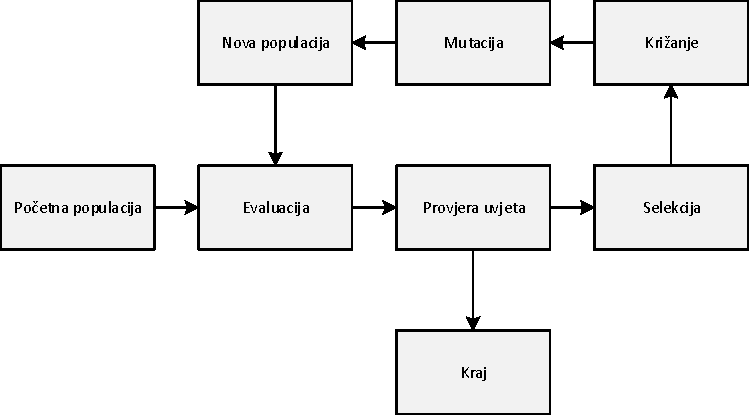
\includegraphics[width=0.7\textwidth]{Images/Gen.pdf}
    \captionsetup{justification=centering}
    \caption{Slijed rada generacijskog genetskog algoritma \cite{optjava}}
    \label{fig:gen}
\end{figure}

\subsubsection{Kromosom}
Kromosom korišten u genetskom algoritmu modelira jednu jedinku, odnosno služi kao reprezentacija jednog rješenja.
Kako se algoritam koristi u svrhu treniranja neuronske mreže, kromosom je predstavljen nizom realnih brojeva koji odgovaraju težinama ulaza neurona neuronske mreže.

\subsubsection{Evaluacija}
Prilikom evaluacije je potrebno odrediti koliko je određena jedinka uspješna, što se u ovom slučaju mjeri kao postotak uspješno klasificiranih podataka iz skupa podataka za treniranje.
Skup za treniranje sastoji se od $15910$ slika veličine $75x75$ slikovnih elemenata.
Slike su unutar skupa podijeljene na $10$ kategorija gdje svaka od njih predstavlja po jednu moguću vrijednost vrha ćelije kako je prikazano na slici \ref{fig:corners}, te kategorije u kojoj se nalaze sve one slike koje na sebi ne sadrže element tablice.
Dobrota jedinke prvotno je bila definirana samo kao postotak uspješno klasificiranih slika.
Takav pristup je imao problema uzrokovanih neproporcionalnim količinama podataka svake od kategorije (primjerice postoji $13950$ slika koje nisu elementi tablice), zbog čega je jedinka mogla imati velik postotak uspješnosti tako da sve klasificira kao nešto što nije element tablice.
Taj je problem moguće riješiti povećanjem skupa za treniranje, što nije jednostavno izvedivo.
Drugo rješenje koje je i iskorišteno u ovom slučaju je promjena evaluacijske funkcije tako da računa postotak uspješne klasifikacije za svaku pojedinu kategoriju podataka te kao konačan rezultat koristi aritmetičku sredinu tako dobivenih postotaka.
 
\subsubsection{Selekcija}
U koraku selekcije potrebno je odabrati dvije jedinke koje će biti korištene u daljnjem postupku križanja kako bi se stvorila nova jedinka.
Postoje različiti postupci selekcija, a cilj istih je mogućnost utjecanja na to koje će jedinke stvarati potomstvo. 
Ako se uvijek biraju samo najbolje jedinke, populacija kroz samo nekoliko generacija u potpunosti gubi genetsku raznolikost zbog čega lako zapinje u lokalnim optimumima.
S druge strane, ako se sve jedinke biraju nasumično s jednakom vjerojatnošću, populacija neće napredovati te algoritam neće konvergirati ka boljim rješenjima.\\
Kako bi se ostvario balans između navedena dva načina odabira, u implementaciji su korištena $2$ načina selekcije roditelja.
Prvi roditelj se bira nasumično, gdje svaka jedinka ima jednaku vjerojatnost biti odabrana.
Drugi roditelj se bira korištenjem turnirske selekcije, koja odabire određen broj potencijalnih roditelja (u ovom slučaju je korištena veličina turnira $3$) te od tako nasumično odabranih roditelja odabire onoga s najvećom funkcijom dobrote.

\subsubsection{Križanje}
Nakon što su odabrani roditelji provodi se križanje. 
U ovom je koraku potrebno stvoriti novu jedinku kombinacijom genetskog materijala roditelja. 
Kao i u prethodnom koraku i ovdje se javlja problem mogućnosti konvergiranja rješenja u lokalni optimum te postoje različiti pristupi kojima je moguće efikasno izvesti ovu operaciju.
U ovom radu korišteno je križanje BLX-$\alpha$ koje radi na način da svaku vrijednost određuje kao slučajnu vrijednost uniformne distribucije u intervalu vrijednosti roditelja kako je prikazano na slici \ref{fig:blx}, a što je detaljno opisano u knjizi \cite{GeneticAlgorithms}. 
Kako bi se smanjilo sažimanje populacije, interval iz kojega se bira vrijednost pojedinog elementa djeteta se proširuje za $\alpha$ posto, čime se omogućava dobivanje rješenja različitih od roditelja.

\begin{figure}[ht!]
    \centering
    \includegraphics[width=0.7\textwidth]{Images/Blx-a.pdf}
    \captionsetup{justification=centering}
    \caption{Primjer rada BLX-$\alpha$ križanja}
    \label{fig:blx}
\end{figure}

\subsubsection{Mutacija}
Prilikom mutacije je potrebno promijeniti vrijednosti kromosoma koje su dobivene križanjem roditelja kako bi se uvela nova genetska raznolikost u populaciju.
Korištena je mutacija koja uz vjerojatnost od $0.05\%$ određeni element kromosoma tako da mu doda nasumičnu vrijednost iz normalne distribucije, pomnoženu sa $0.5$. 

\subsubsection{Rezultati}
\begin{figure}[ht!]
    \centering
    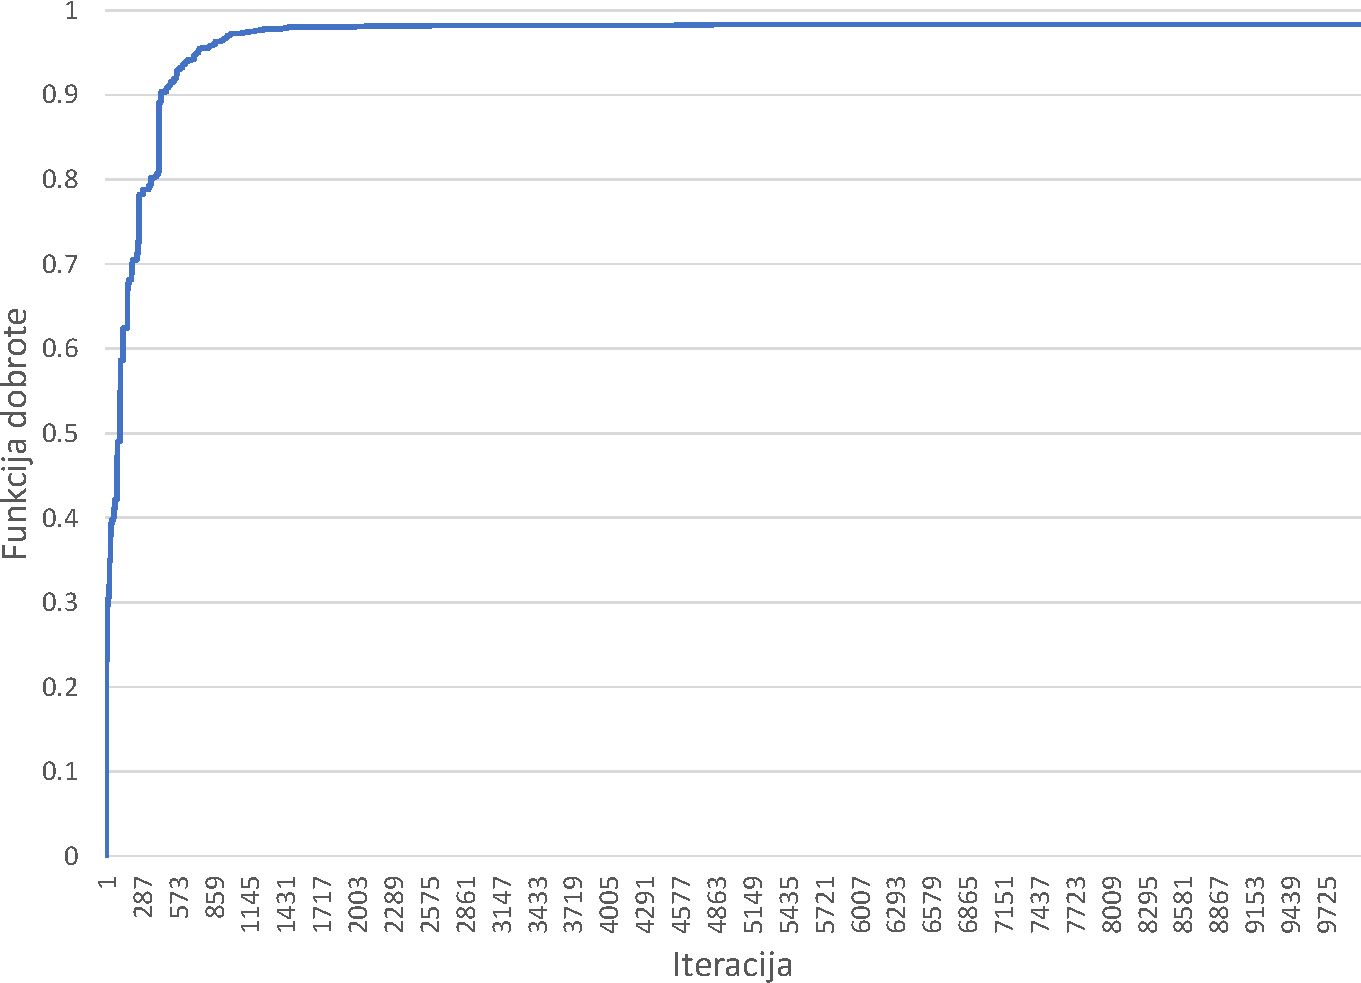
\includegraphics[width=0.85\textwidth]{Images/Ga.pdf}
    \captionsetup{justification=centering}
    \caption{Rezultati izvođenja genetskog algoritma}
    \label{fig:ga}
\end{figure}

Opisana neuronska mreža ima $500$ težina koje je potrebno postaviti, što znači da genetski algoritam radi s kromosomima duljine $500$. 
Na slici \ref{fig:ga} prikazana je vrijednost najbolje jedinke pronađene genetskim algoritmom u odnosu na iteraciju algoritma.
Vidljivo je kako populacija na početnu brzo napreduje, no pretraga se s vremenom usporava te algoritam ne uspijeva postići zadovoljavajuće razine točnosti.

\subsection{Treniranje korištenjem algoritma propagacije pogreške unatrag}
Drugi pristup treniranju neuronske mreže je korištenje algoritma propagacije pogreške unatrag koji je detaljno opisan u knjizi \cite{neuroracunarstvo}.
Za razliku od genetskog algoritma koji nema nikakvo znanje o tome u kojem smjeru se nalazi optimalno rješenje, ovaj algoritam računa odstupanja dobivenog rezultata od očekivanog za svaki neuron te primjenom gradijentnog spusta podešava težine kako bi smanjio pogrešku.
U ovom radu korištena je stohastička verzija navedenog algoritma koja težine ažurira na temelju greške nastale na samo jednom primjeru iz testnog skupa, a što je detaljnije objašnjeno u nastavku.


\subsubsection{Izračun pogreške}
Označimo li sa $t_o$ očekivani izlaz neuronske mreže za neuron $o$ za trenutni podatak te sa $y_o^{(k + 1)}$ stvarni izlaz neurona, greška neuronske mreže $E$ definirana je kao suma kvadratnih odstupanja, odnosno kao:
\[
    E = \frac{1}{2}\sum(t_o-y_o^{(k + 1)})^2
\]
Kako bi se ostvario gradijentni spust, potrebno je izračunati gradijent pogreške za svaku težinu $w_{ij}^{(k)}$, što označava težinu koja spaja $i$-ti neuron u sloju $k$ sa $j$-tim neuronom u sloju $k+1$:
\[
    \frac{\partial E}{\partial w_{ij}^{(k)}}
\]
Tada se težina ažurira kao:
\[
    w_{ij}^{(k)} \leftarrow w_{ij}^{(k)} - \alpha \frac{\partial E}{\partial w_{ij}^{(k)}}
\]
gdje je $\alpha$ mala pozitivna konstanta poznata kao stopa učenja.

\subsubsection{Gradijent izlaznog sloja}
Potrebno je izračunati $\frac{\partial E}{\partial w_{ij}^{(k)}}$, što se može zapisati kao:
\begin{equation*}
\begin{split}
    \frac{\partial E}{\partial w_{ij}^{(k)}}
        & = \frac{\partial}{\partial w_{ij}^{(k)}} 
        \left[\frac{1}{2}\displaystyle\sum_{o = 1}^m(t_o - y_o^{(k + 1)})^2\right]\\
        & = \frac{1}{2} \displaystyle\sum_{o = 1}^m2(t_o - y_o^{(k + 1)})(-1) \frac{\partial y_o^{(k + 1)}}{\partial w_{ij}^{(k)}} \\
        & = -\displaystyle\sum_{o = 1}^m(t_o - y_o^{(k + 1)})\frac{\partial y_o^{(k + 1)}}{\partial w_{ij}^{(k)}}
\end{split}
\end{equation*}

Pritom težina $w_{ij}^{(k)}$ spaja $i$-ti neuron sloja $k$ sa $j$-tim neuronom sloja $k+1$ i nema utjecaja na ostale neurone, zbog čega su parcijalne derivacije $\frac{\partial y_o^{(k + 1)}}{\partial w_{ij}^{(k)}} = 0$ za $o != j$ pa se jednadžba može zapisati kao:

\[
    \frac{\partial E}{\partial w_{ij}^{(k)}}
    = -(t_j - y_j^{(k + 1)})\frac{\partial y_j^{(k + 1)}}{\partial w_{ij}^{(k)}}
\]
Korištenjem lančanog pravila, parcijalna derivacija iz izraza se može zapisati kao:
\[
    \frac{\partial y_j^{(k + 1)}}{\partial w_{ij}^{(k)}}
    = \frac{\partial y_j^{(k + 1)}}{\partial net_{j}^{(k+1)}}
    \frac{\partial net_{j}^{(k+1)}}{\partial w_{ij}^{(k)}}
\]
gdje je sa $net_{j}^{(k+1)}$ označena težinska suma za neuron $j$ sloja $k+1$. Kako se koriste sigmoidalna aktivacijska funkcija, vrijedi da je:
\[
    \frac{\partial y_j^{(k + 1)}}{\partial net_{j}^{(k+1)}}
    = y_j^{(k + 1)} (1 - y_j^{(k + 1)})
\]
Kako vrijedi da je
\[
    net_{j}^{(k+1)} = \displaystyle\sum_o w_{o,j}^{(k)}y_o^{(k)}    
\]
jedini član izraza koji ovisi o težini $w_{ij}^{(k)}$ je $w_{i,j}^{(k)}y_i^{(k)}$ zbog čega je parcijalna derivacija:
\[
    \frac{\partial net_{j}^{(k+1)}}{\partial w_{ij}^{(k)}} = y_i^{(k)}
\]
Uvrštavanjem dobivenog izraza u početnu jednadžbu dobiva se:
\[
    \frac{\partial E}{\partial w_{ij}^{(k)}}
    = -(t_j - y_j^{(k + 1)})
    y_j^{(k + 1)} (1 - y_j^{(k + 1)})
    y_i^{(k)}
\]
Radi jednostavnosti se greška $j$-tog neorona za dani primjer za učenje označava sa $\delta_j^{(k+1)}$ te vrijedi:
\[
    \delta_j^{(k+1)} = y_j^{(k + 1)}(1 - y_j^{(k + 1)})(t_j - y_j^{(k + 1)})
\]
Te se sada parcijalna derivacija ukupne greške može prikazati kao:
\[
    \frac{\partial E}{\partial w_{ij}^{(k)}} = -\delta_j^{(k+1)}y_i^{(k)}
\]

\subsubsection{Gradijent skrivenog sloja}
Potrebno je izračunati $\frac{\partial E}{\partial w_{ij}^{(k-1)}}$, što se može zapisati kao:
\begin{equation*}
\begin{split}
    \frac{\partial E}{\partial w_{ij}^{(k-1)}}
        & = \frac{\partial}{\partial w_{ij}^{(k-1)}} 
        \left[\frac{1}{2}\displaystyle\sum_{o = 1}^m(t_o - y_o^{(k + 1)})^2\right]\\
        & = \frac{1}{2} \displaystyle\sum_{o = 1}^m2(t_o - y_o^{(k + 1)})(-1) \frac{\partial y_o^{(k + 1)}}{\partial w_{ij}^{(k-1)}} \\
        & = -\displaystyle\sum_{o = 1}^m(t_o - y_o^{(k + 1)})\frac{\partial y_o^{(k + 1)}}{\partial w_{ij}^{(k-1)}}\\
        & = -\displaystyle\sum_{o = 1}^m(t_o - y_o^{(k + 1)})\frac{\partial y_o^{(k + 1)}}{\partial net_{o}^{(k+1)}}\frac{\partial net_o^{(k + 1)}}{\partial w_{ij}^{(k-1)}}
\end{split}
\end{equation*}
Prva parcijalna derivacija je derivacija sigmoidalne funkcije što je:
\[
    \frac{\partial y_o^{(k + 1)}}{\partial net_{o}^{(k+1)}}
    = y_o^{(k + 1)} (1 - y_o^{(k + 1)})
\]
Uvrštavanjem izračunatog u početni izraz dobiva se:
\begin{equation*}
\begin{split}
    \frac{\partial E}{\partial w_{ij}^{(k-1)}}
        & = -\displaystyle\sum_{o = 1}^m(t_o - y_o^{(k + 1)})y_o^{(k + 1)} (1 - y_o^{(k + 1)})\frac{\partial net_o^{(k + 1)}}{\partial w_{ij}^{(k-1)}}\\
        & = -\displaystyle\sum_{o = 1}^m\delta_o^{(k+1)}\frac{\partial net_o^{(k + 1)}}{\partial w_{ij}^{(k-1)}}
\end{split}
\end{equation*}
Druga parcijalna derivacija računa se pomoću $net_o^{(k + 1)}$ koji se može zapisati kao:
\[
    net_o^{(k + 1)} = \displaystyle\sum_l w_{l,o}^{(k)}y_l^{(k)}
\]
Kako je potrebno izračunati parcijalnu derivaciju za težinu $w_{ij}^{(k-1)}$ valja uočiti da ta težina utječe samo na vrijednost neurona $j$ u sloju $k$ odnosno na vrijednost $y_j^{(k)}$, zbog čega vrijedi:
\[
    \frac{\partial net_o^{(k + 1)}}{\partial w_{ij}^{(k-1)}}
    = w_{j,o}^{(k)}\frac{\partial y_j^{(k)}}{\partial w_{ij}^{(k-1)}}
\]
Parcijalna derivacija $\frac{\partial y_j^{(k)}}{\partial w_{ij}^{(k-1)}}$ rješava se na jednak način kao i u izlaznom sloju te vrijedi:
\begin{equation*}
\begin{split}
    \frac{\partial y_j^{(k)}}{\partial w_{ij}^{(k-1)}}
        & = \frac{\partial y_j^{(k)}}{\partial net_{j}^{(k)}}
            \frac{\partial net_{j}^{(k)}}{\partial w_{ij}^{(k-1)}}\\
        & = y_j^{(k)} (1 - y_j^{(k)}) y_i^{(k - 1)}
\end{split}
\end{equation*}
Uvrštavanjem u prethodnu jednakost slijedi:
\[
    \frac{\partial net_o^{(k + 1)}}{\partial w_{ij}^{(k-1)}}
        = w_{j,o}^{(k)}y_j^{(k)} (1 - y_j^{(k)}) y_i^{(k - 1)}
\]
Što vraćanjem u početnu jednakost daje:
\begin{equation*}
\begin{split}
    \frac{\partial E}{\partial w_{ij}^{(k-1)}}
        & = -\displaystyle\sum_{o = 1}^m\delta_o^{(k+1)}w_{j,o}^{(k)}y_j^{(k)} (1 - y_j^{(k)}) y_i^{(k - 1)}\\
        & = -y_i^{(k - 1)} y_j^{(k)} (1 - y_j^{(k)})\displaystyle\sum_{o = 1}^m\delta_o^{(k+1)}w_{j,o}^{(k)}
\end{split}
\end{equation*}
Ponovno se uvodi oznaka $\delta_j^{k}$ za grešku neurona, koja je definirana kao:
\[
    \delta_j^{k} = y_j^{(k)} (1 - y_j^{(k)})\displaystyle\sum_{o = 1}^m\delta_o^{(k+1)}w_{j,o}^{(k)} 
\]
Te se sada konačni rezultat može zapisati kao:
\[
    \frac{\partial E}{\partial w_{ij}^{(k-1)}} =
    -y_i^{(k - 1)}\delta_j^{k}
\]

\subsubsection{Rezultati}
\begin{figure}[ht!]
    \centering
    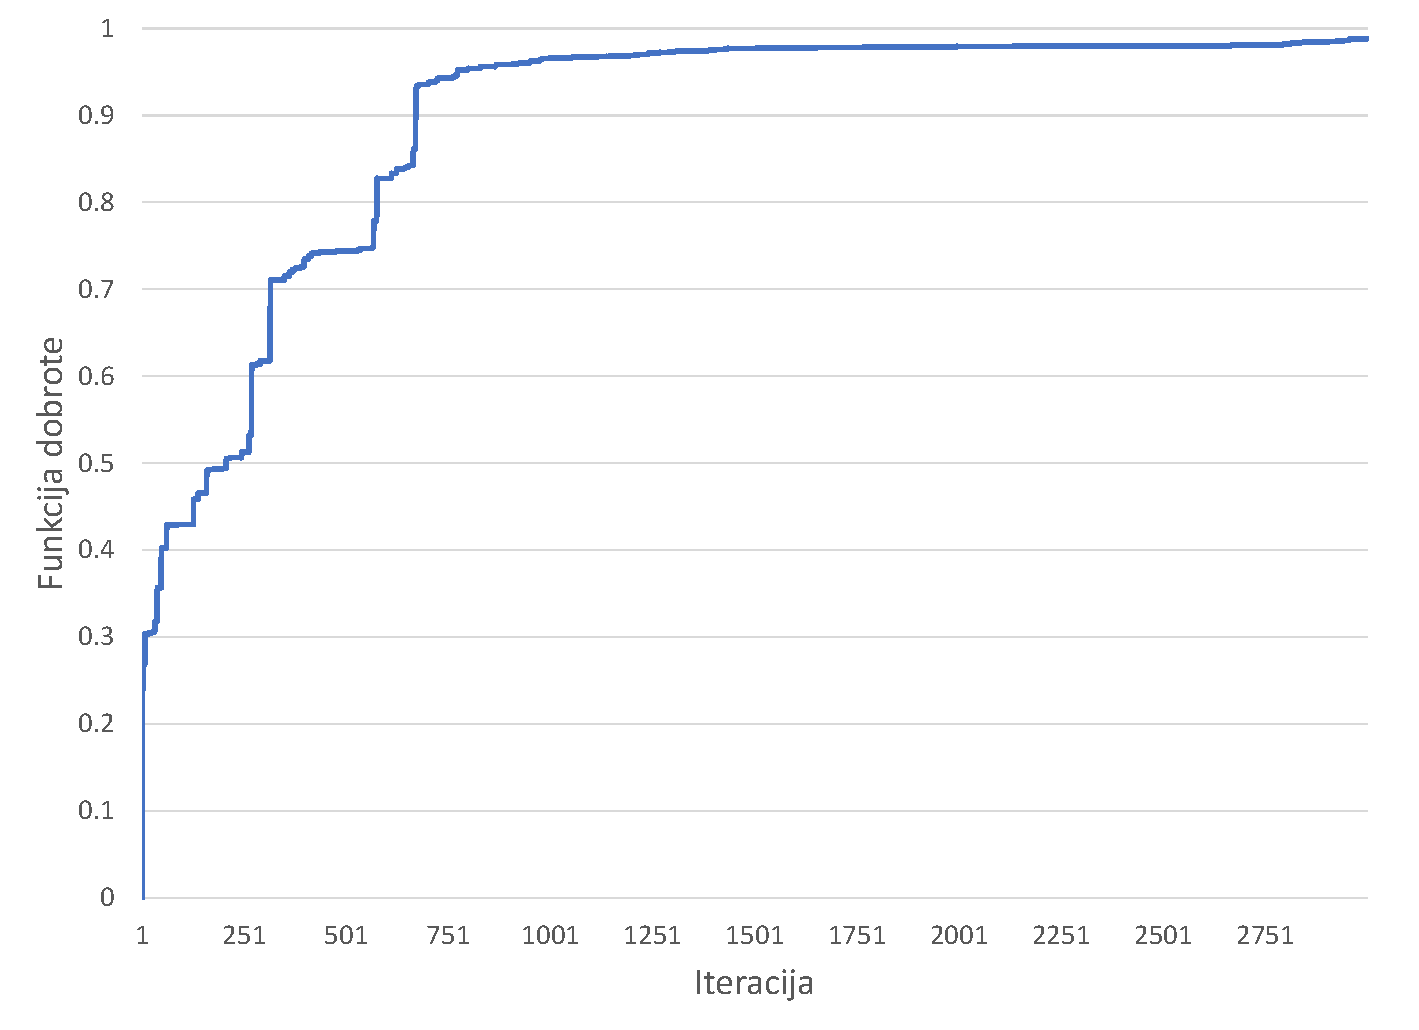
\includegraphics[width=0.85\textwidth]{Images/Backprop.pdf}
    \captionsetup{justification=centering}
    \caption{Rezultati izvođenja algoritma backpropagation}
    \label{fig:backprop}
\end{figure}

Primjena ovako opisanog algoritma stvara probleme zbog činjenice da se broj podataka za pojedine kategorije skupa za učenje drastično razlikuju.
To je riješeno tako da se prilikom ažuriranja vrijednosti težine, osim sa stopom učenja podatak množi i s konstantom koja je obrnuto proporcionalna broju uzoraka za trenutnu kategoriju podatka.
Vidljivo je kako u početnim iteracijama algoritma postotak točne klasifikacije korištenjem algoritma backpropagation raste približno slično rastu funkcije dobrote genetskog algoritma.
Najveća razlika je uočiva kod vrijednosti koje prepoznaju više od $0.9$ podataka točno.
Kod ovog algoritma takve se neuronske mreže i dalje unaprjeđuju što je vidljivo blagim nagibom krivulje na slici \ref{fig:backprop}.
Za razliku od genetskog algoritma, ovaj algoritam uspijeva doći do vrijednosti od preko $0.99$ na testu za učenje.

\section{Algoritam AdaBoost}
Za potrebe ovog klasifikacijskog algoritma potrebno je odrediti način na koji se uče slabi klasifikatori.
Svaki slabi klasifikator sastoji se od značajke, praga, konstante $p$ koja određuje vrstu nejednakosti te vrijednosti $\alpha$ koja određuje koliko je klasifikator značajan, odnosno koliko njegov izlaz doprinosi konačnoj odluci jakog klasifikatora.
Vrijednost $\alpha$ računa se na temelju ostalih argumenata klasifikatora na skupu podataka za treniranje koji je jednak skupu podataka korištenom prilikom treniranja umjetne neuronske mreže.
Ostale parametre je potrebno odabrati tako da se minimizira pogreška klasifikatora, što je učinjeno tako da se nasumično odabere značajka koja će se koristiti te se ona inicijalizira s nasumično odabranim vrijednostima.
Ostali parametri također su nasumično odabrani te se za tako dobiven klasifikator računa težinska pogreška na skupu podataka za učenje.
Postupak se ponavlja velik broj puta kako bi se dobio klasifikator s čim manjom pogreškom, koji se koristi prilikom izrade jakog klasifikatora.
\begin{figure}[ht!]
    \centering
    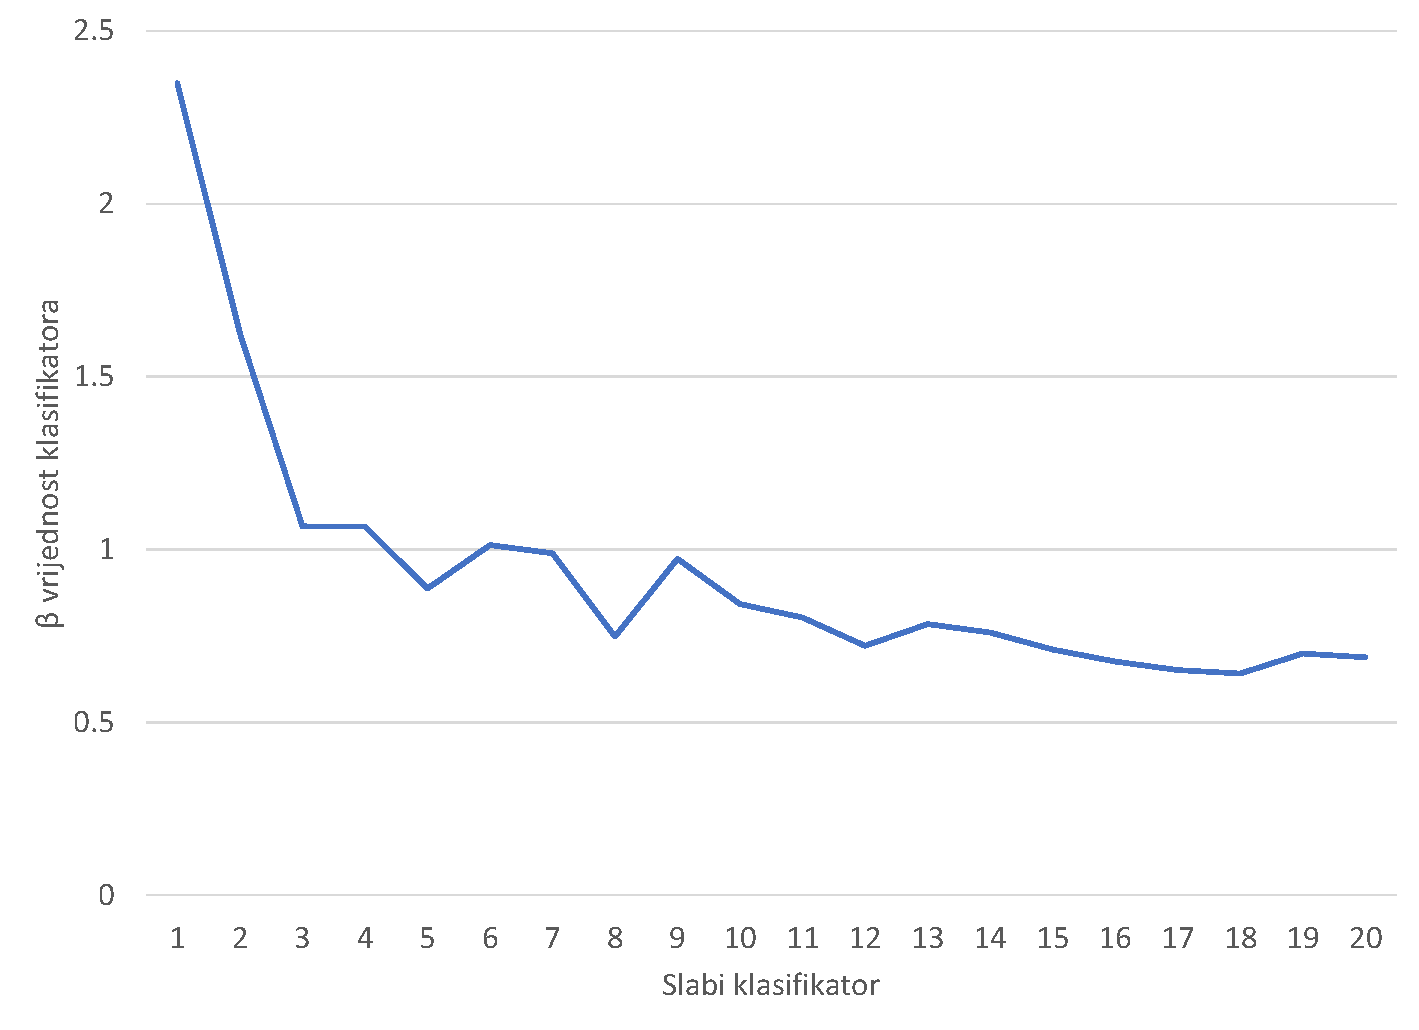
\includegraphics[width=0.85\textwidth]{Images/Ada.pdf}
    \captionsetup{justification=centering}
    \caption{$\alpha$ vrijednosti pojedinih slabih klasifikatora}
    \label{fig:ada}
\end{figure}

Graf na slici \ref{fig:ada} prikazuje $\alpha$ vrijednosti za slabe klasifikatore korištene u izradi jakog klasifikatora. 
Evidentno je kako najveću $\alpha$ vrijednost, a time i najveći doprinos u klasifikaciji ima prvi slabi klasifikator. 
Svaki sljedeći klasifikator u pravilu ima sve manju $\alpha$ vrijednost, kao što je i očekivano zbog toga što je preostale podatke sve teže i teže točno klasificirati. 
Zbog trenda pada doprinosa svakog sljedećeg klasifikatora moguće je jaki klasifikator izgraditi korištenjem prvih nekoliko slabih klasifikatora (u ovom slučaju korišteno je $20$ slabih klasifikatora), jer je sigurno da sljedeći klasifikator neće značajno doprinijeti ukupnom rezultatu, premda će usporiti pretragu.

\section{Usporedba rezultata}

\subsection{Detekcija vrhova ćelija}
Implementirani algoritmi testirani su na skupu podataka koji se sastoji od $216$ ručno ispunjenih tablica, koje su korištene za stvaranje skupa slika vrhova ćelija koji je korišten kao skup za učenje.
Konačni algoritmi su također testirani na skupu od $2266$ slika dobivenih digitalizacijom obrazaca za odgovore ispita, što su podatci za koje je algoritam izrađen.

\begin{figure}[!ht]
    \centering
    \frame{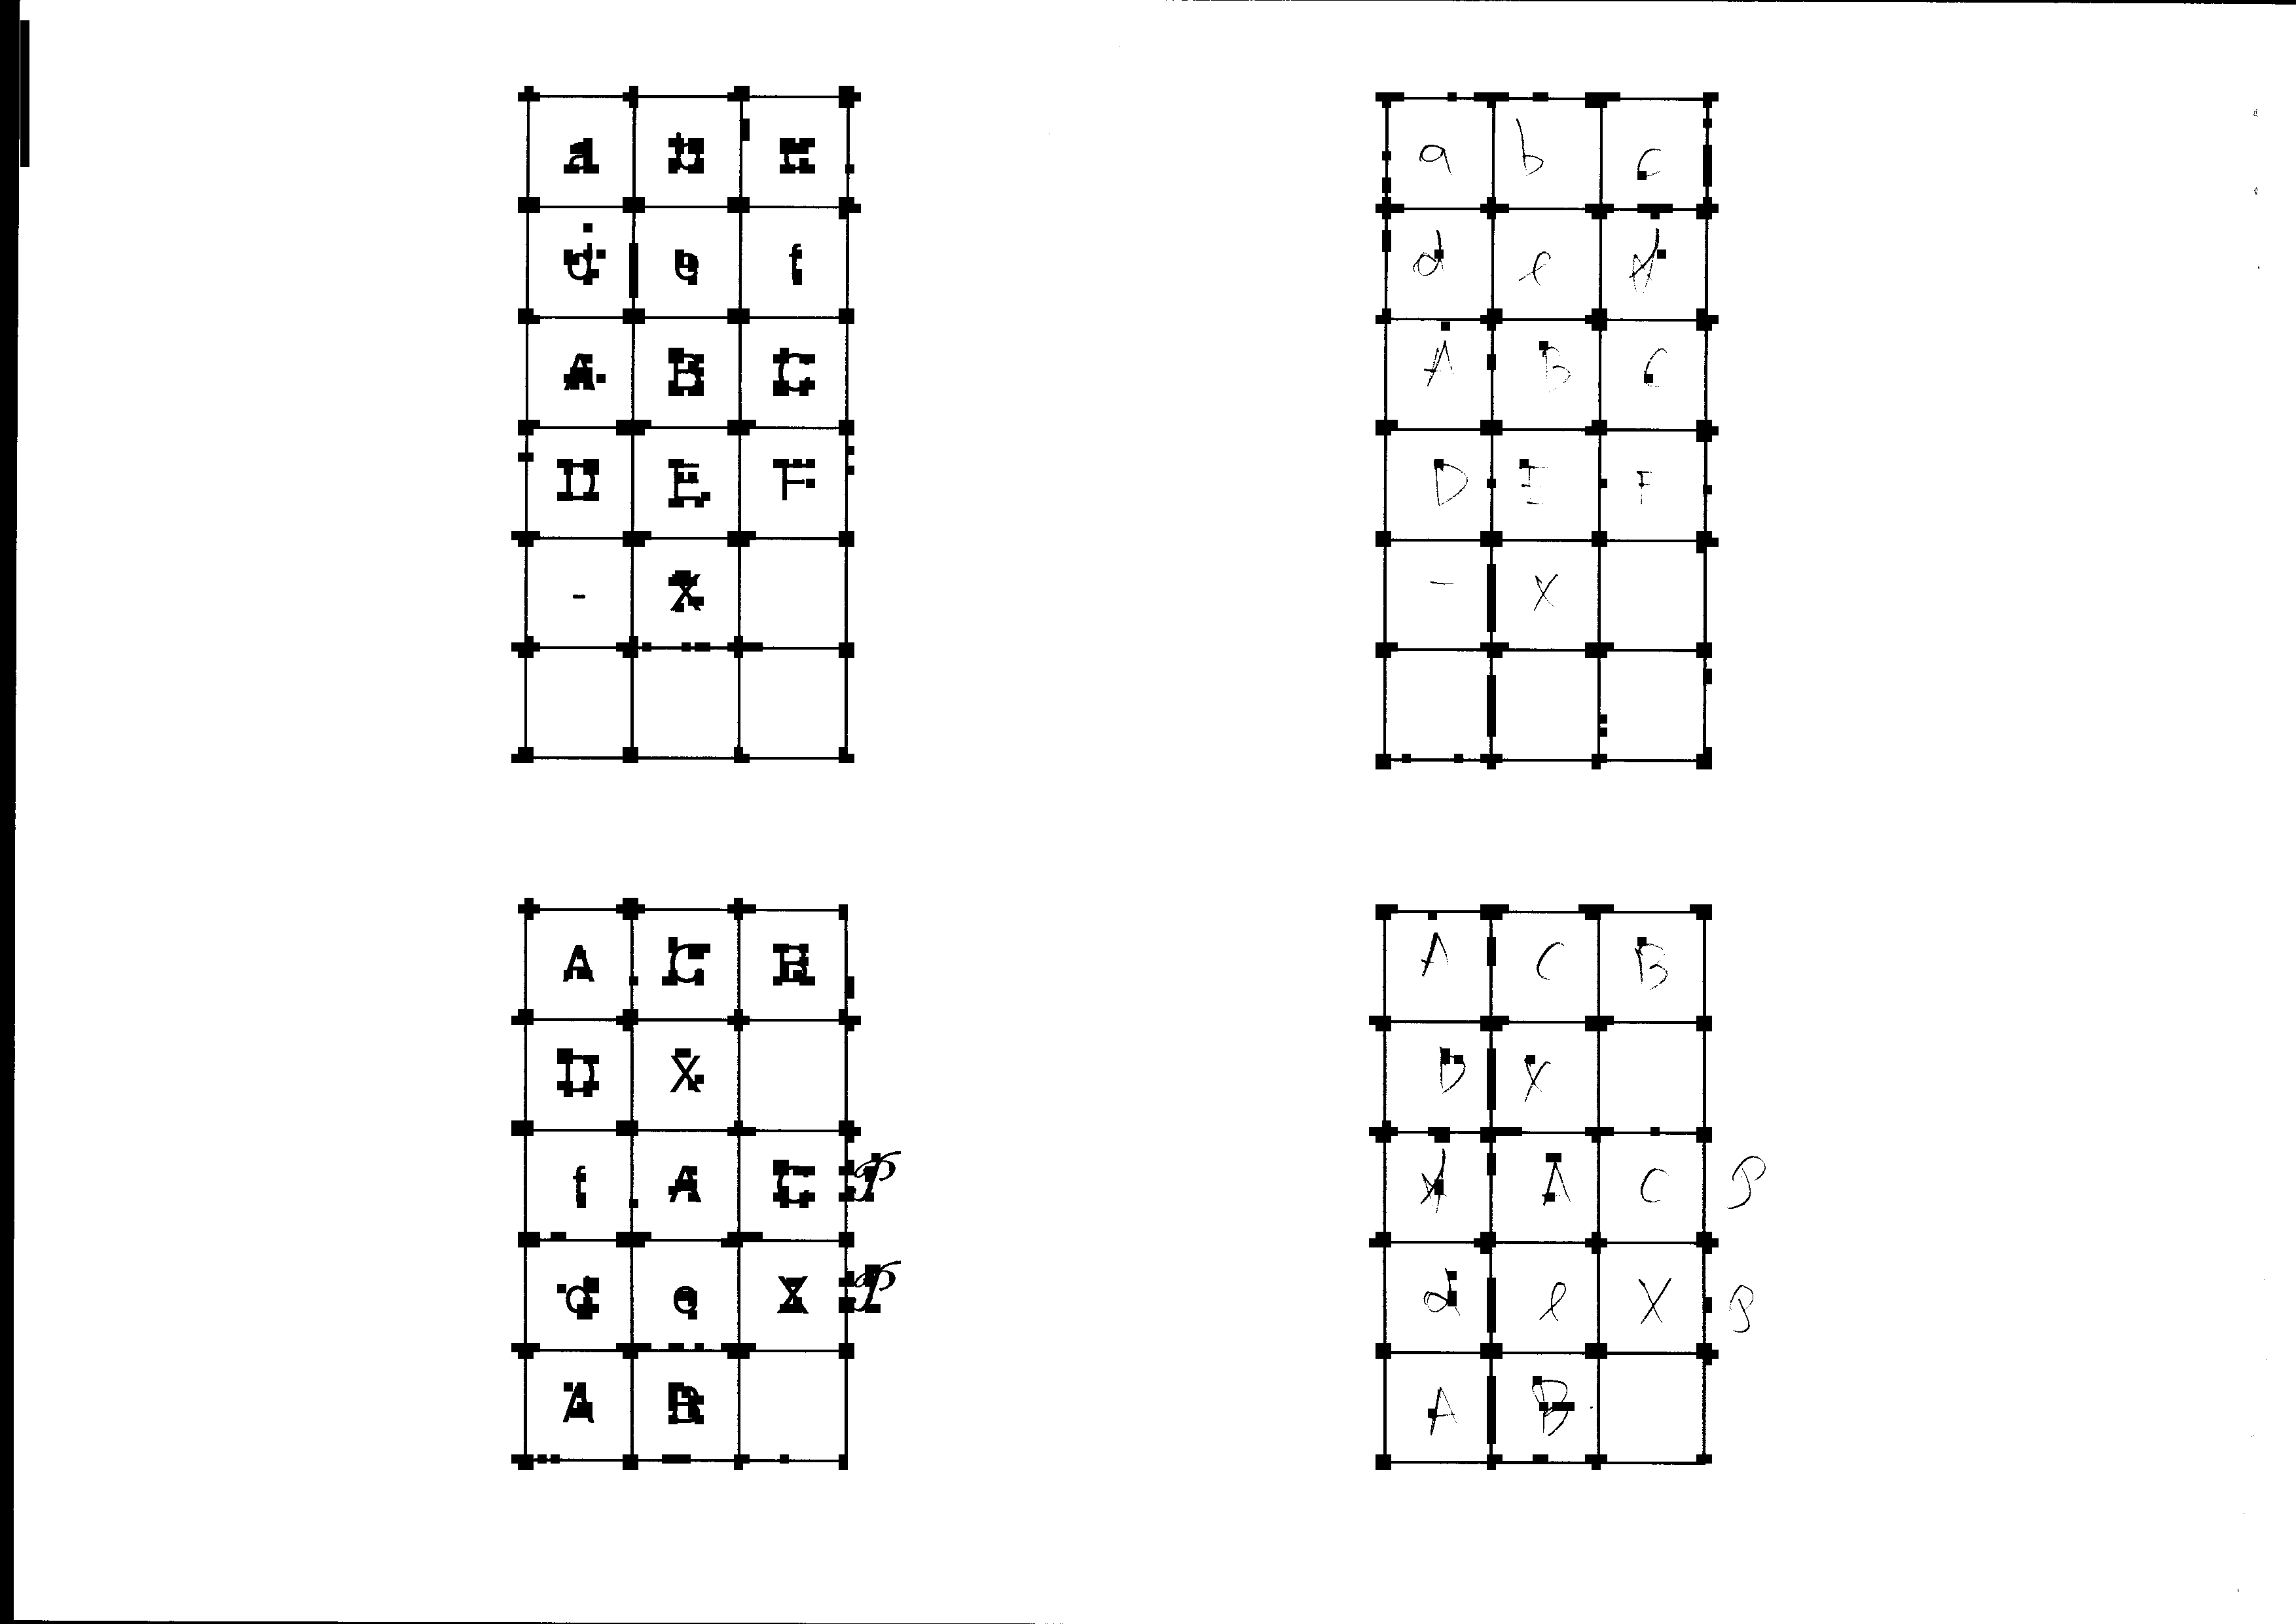
\includegraphics[width=.75\linewidth]{Images/ada.png}}
    \captionsetup{justification=centering}
    \caption{Točke detektirane korištenjem algoritma AdaBoost}
    \label{fig:adaResult}
\end{figure}

Na slici \ref{fig:adaResult} prikazana je slika tablice koja je korištena za potrebe testiranja te su na njoj crnim kvadratima označene pronađene točke.
Primjećuje se da klasifikator uspješno prepoznaje sve točke za koje se očekuje da ih prepozna, ali također prepoznaje i određen broj točaka koje nisu vrhovi ćelija.
Većina krivo prepoznatih točaka nalazi se u tablici s tekstom pisanom na računalu, što je uzrokovano skupom za učenje u kojemu se kao primjeri koje ne treba prepoznati pretežno nalaze primjeri rukom pisanih znakova jer su to primjeri nad kojima algoritam u stvarnosti radi.
Na pogrešku također utječe i činjenica da je jaki klasifikator izgrađen od samo $20$ slabih, premda se na grafu na slici \ref{fig:ada} primjećuje kako trend pada $\alpha$ vrijednosti sugerira kako postoji još slabih klasifikatora koji bi doprinosili konačnom rezultatu.
Unatoč broju grešaka, klasifikator je moguće koristiti jer se njegov izlaz prosljeđuje drugom klasifikatoru čime se ostvaruje veća točnost, zbog čega je u konačnici korišteno rješenje s manjim brojem klasifikatora kako bi se postigla veća brzina.\\

Algoritam je pokrenut na $10$ primjera veličine $3507x2480$ slikovnih elemenata te su zabilježena sljedeća vremena izvođenja: $107.595$, $117.843$, $99.004$, $107.530$, $115.456$, $103.617$, $118.659$, $122.063$, $117.730$, $115.719$, izraženo u milisekundama. 
Prosječno vrijeme izvođenja iznosi $112.5$ms.

\begin{figure}[!ht]
    \centering
    \frame{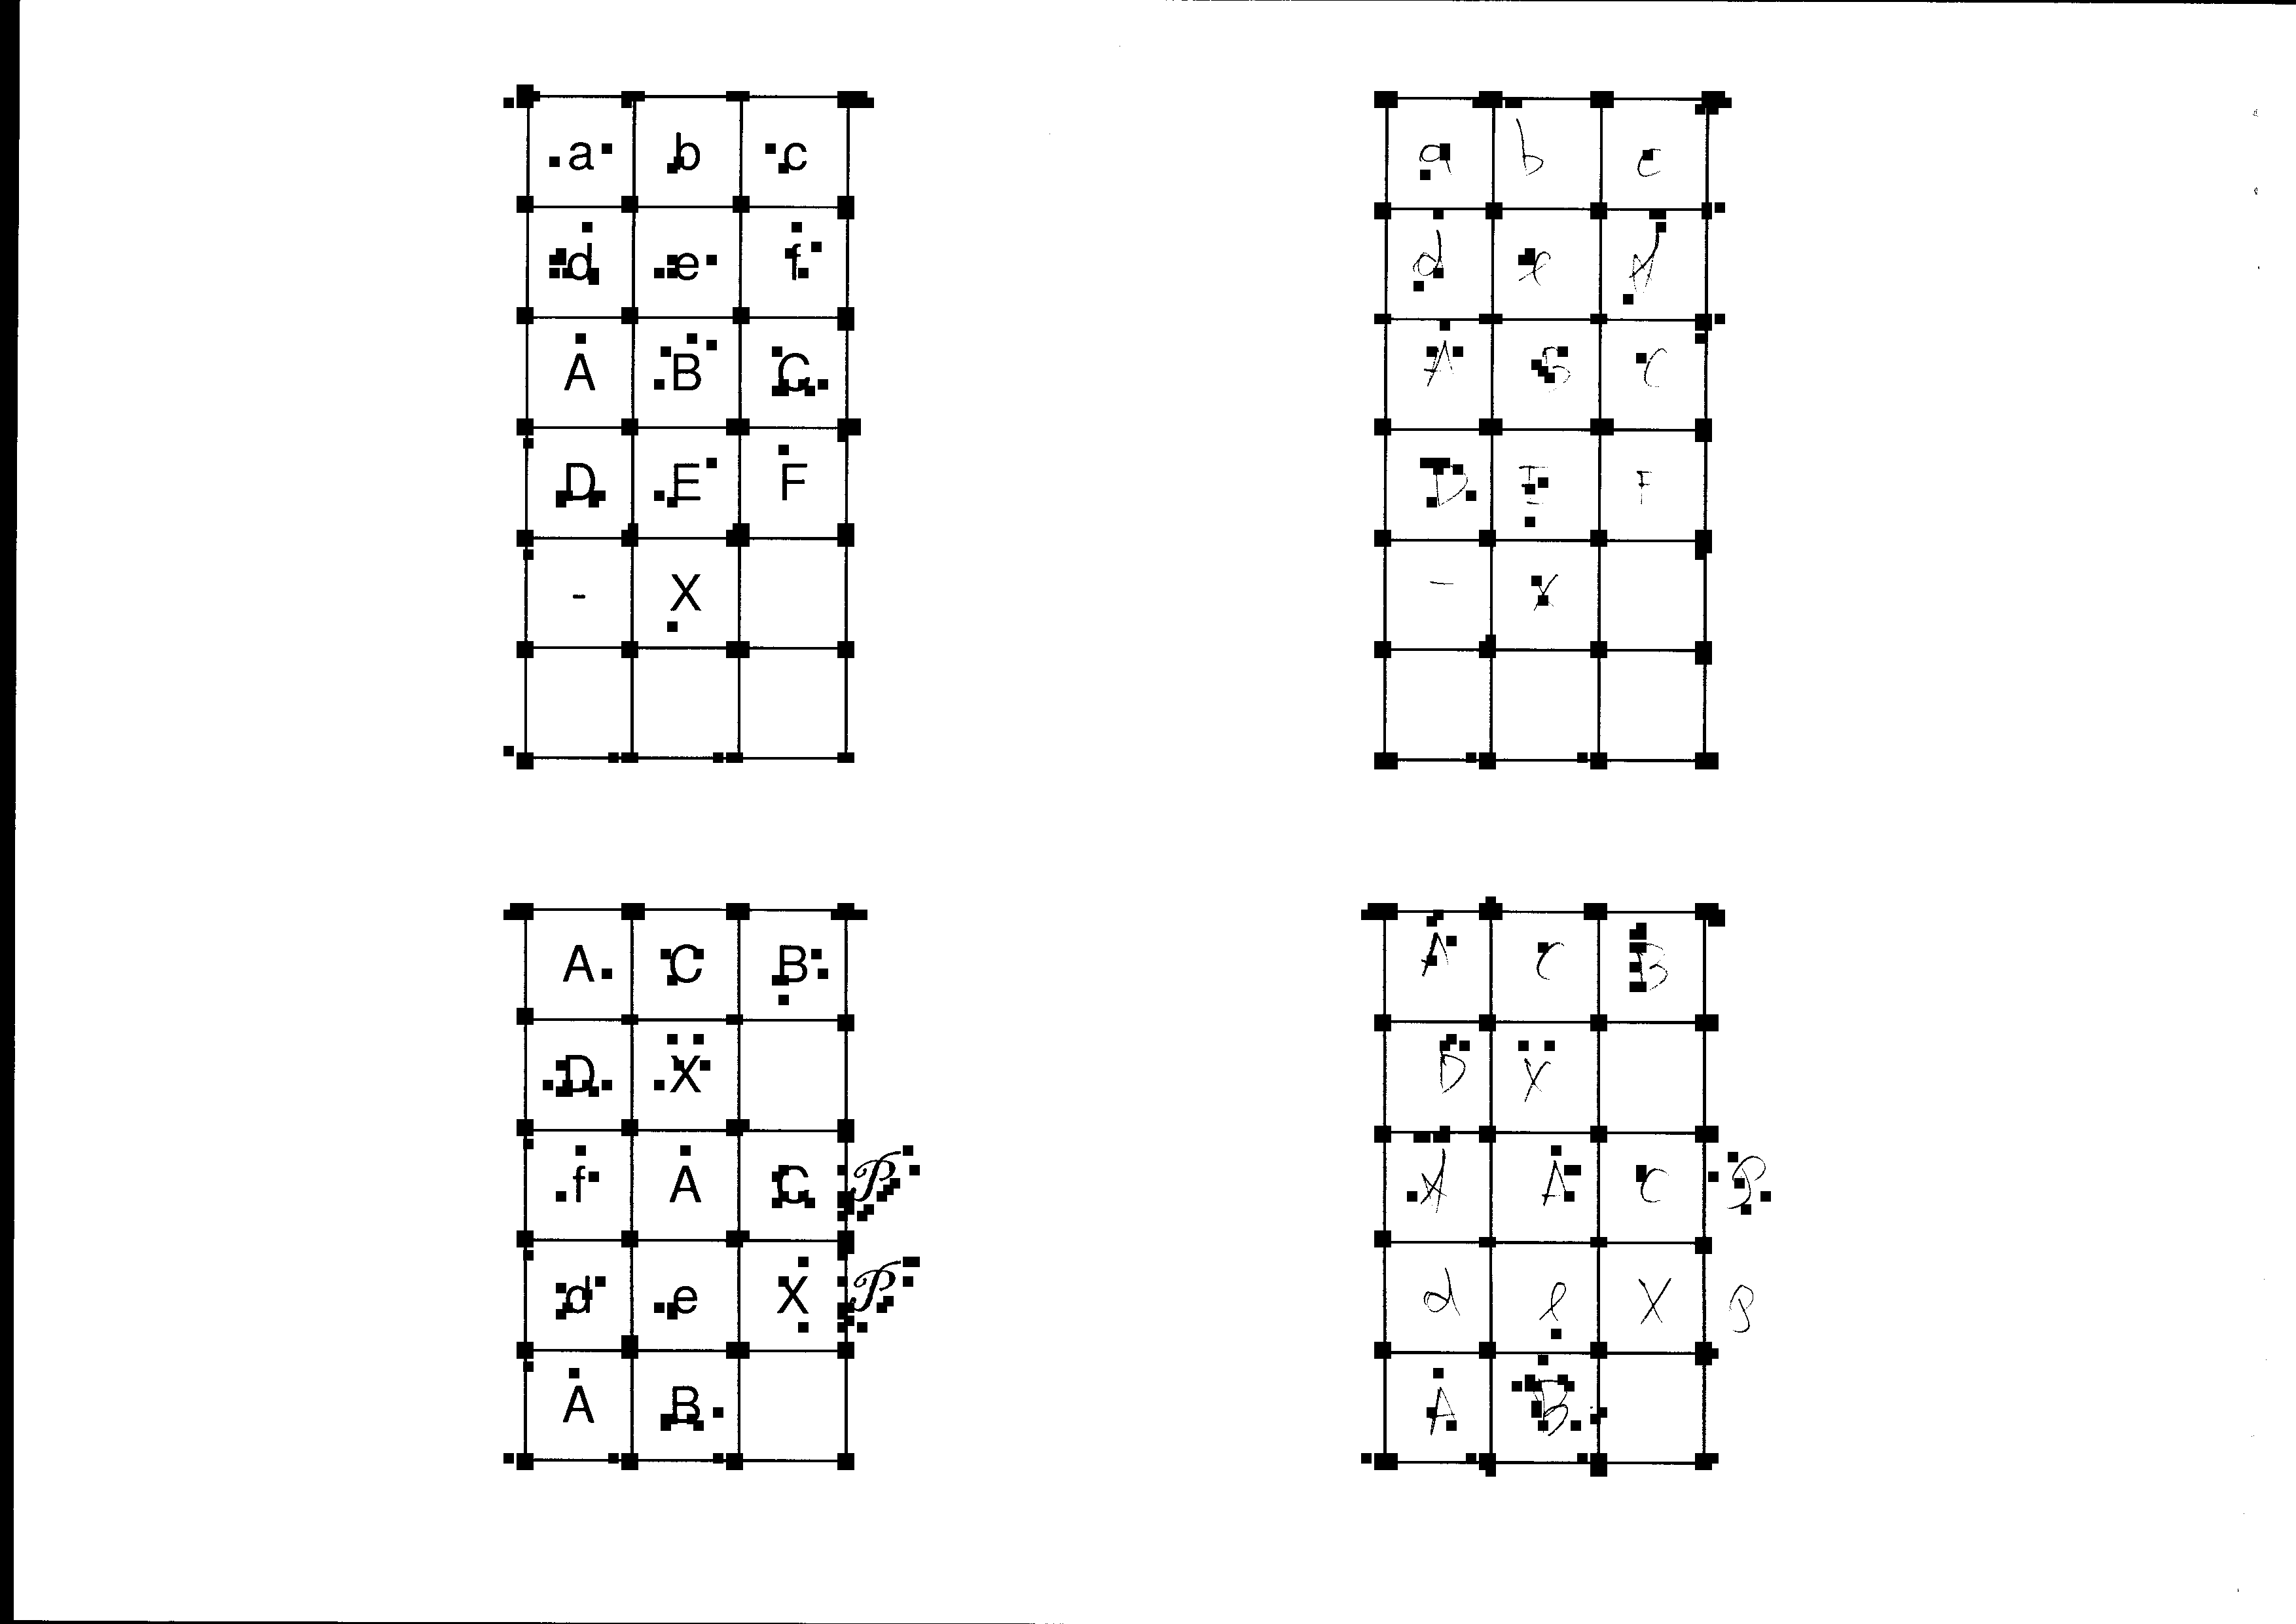
\includegraphics[width=.75\linewidth]{Images/neural.png}}
    \captionsetup{justification=centering}
    \caption{Točke detektirane korištenjem neuronske mreže}
    \label{fig:neuralResult}
\end{figure}

Slika \ref{fig:neuralResult} prikazuje rezultate klasifikacije korištenjem neuronske mreže. 
Također se uočava kako su sve stvarne vrijednosti uspješno prepoznate, ali postoji određen broj točaka koje su prepoznate premda ne bi trebale biti. 
Problem je moguće riješiti promjenom arhitekture neuronske mreže dodavanjem dodatnih neurona ili čak dodavanjem novog skrivenog sloja, ili jednostavno drugačijom definicijom značajki ili dodavanjem novih značajki.
Kako se neuronska mreža koristi nad rezultatima koje daje prethodni klasifikacijski algoritam, dobiveni rezultati pokazuju se zadovoljavajućima.\\

Algoritam je pokrenut na $10$ primjera veličine $3507x2480$ slikovnih elemenata te su zabilježena sljedeća vremena izvođenja: $811.518$, $669.809$, $701.195$, $727.840$, $657.510$, $669.887$, $672.872$, $642.865$, $656.021$, $675.564$, izraženo u milisekundama. 
Prosječno vrijeme izvođenja iznosi $688.5$ms.\\

Primjenom T-testa uz hipoteze $H_0: \mu_1 = \mu_2$ i $H_1: \mu_1 < \mu_2$ uz nivo značajnosti od $\alpha = 0.05$ dobivena je $P$ vrijednost $9.421\cdot10^{-12}$ na temelju čega se hipoteza $H_0$ odbacuje u korist hipoteze $H_1$ čime se zaključuje kako je prosječno vrijeme izvođenja klasifikacije algoritmom AdaBoost statistički značajno manje od prosječnog vremena izvođenja klasificiranja korištenjem umjetne neuronske mreže.

\begin{figure}[!ht]
    \centering
    \frame{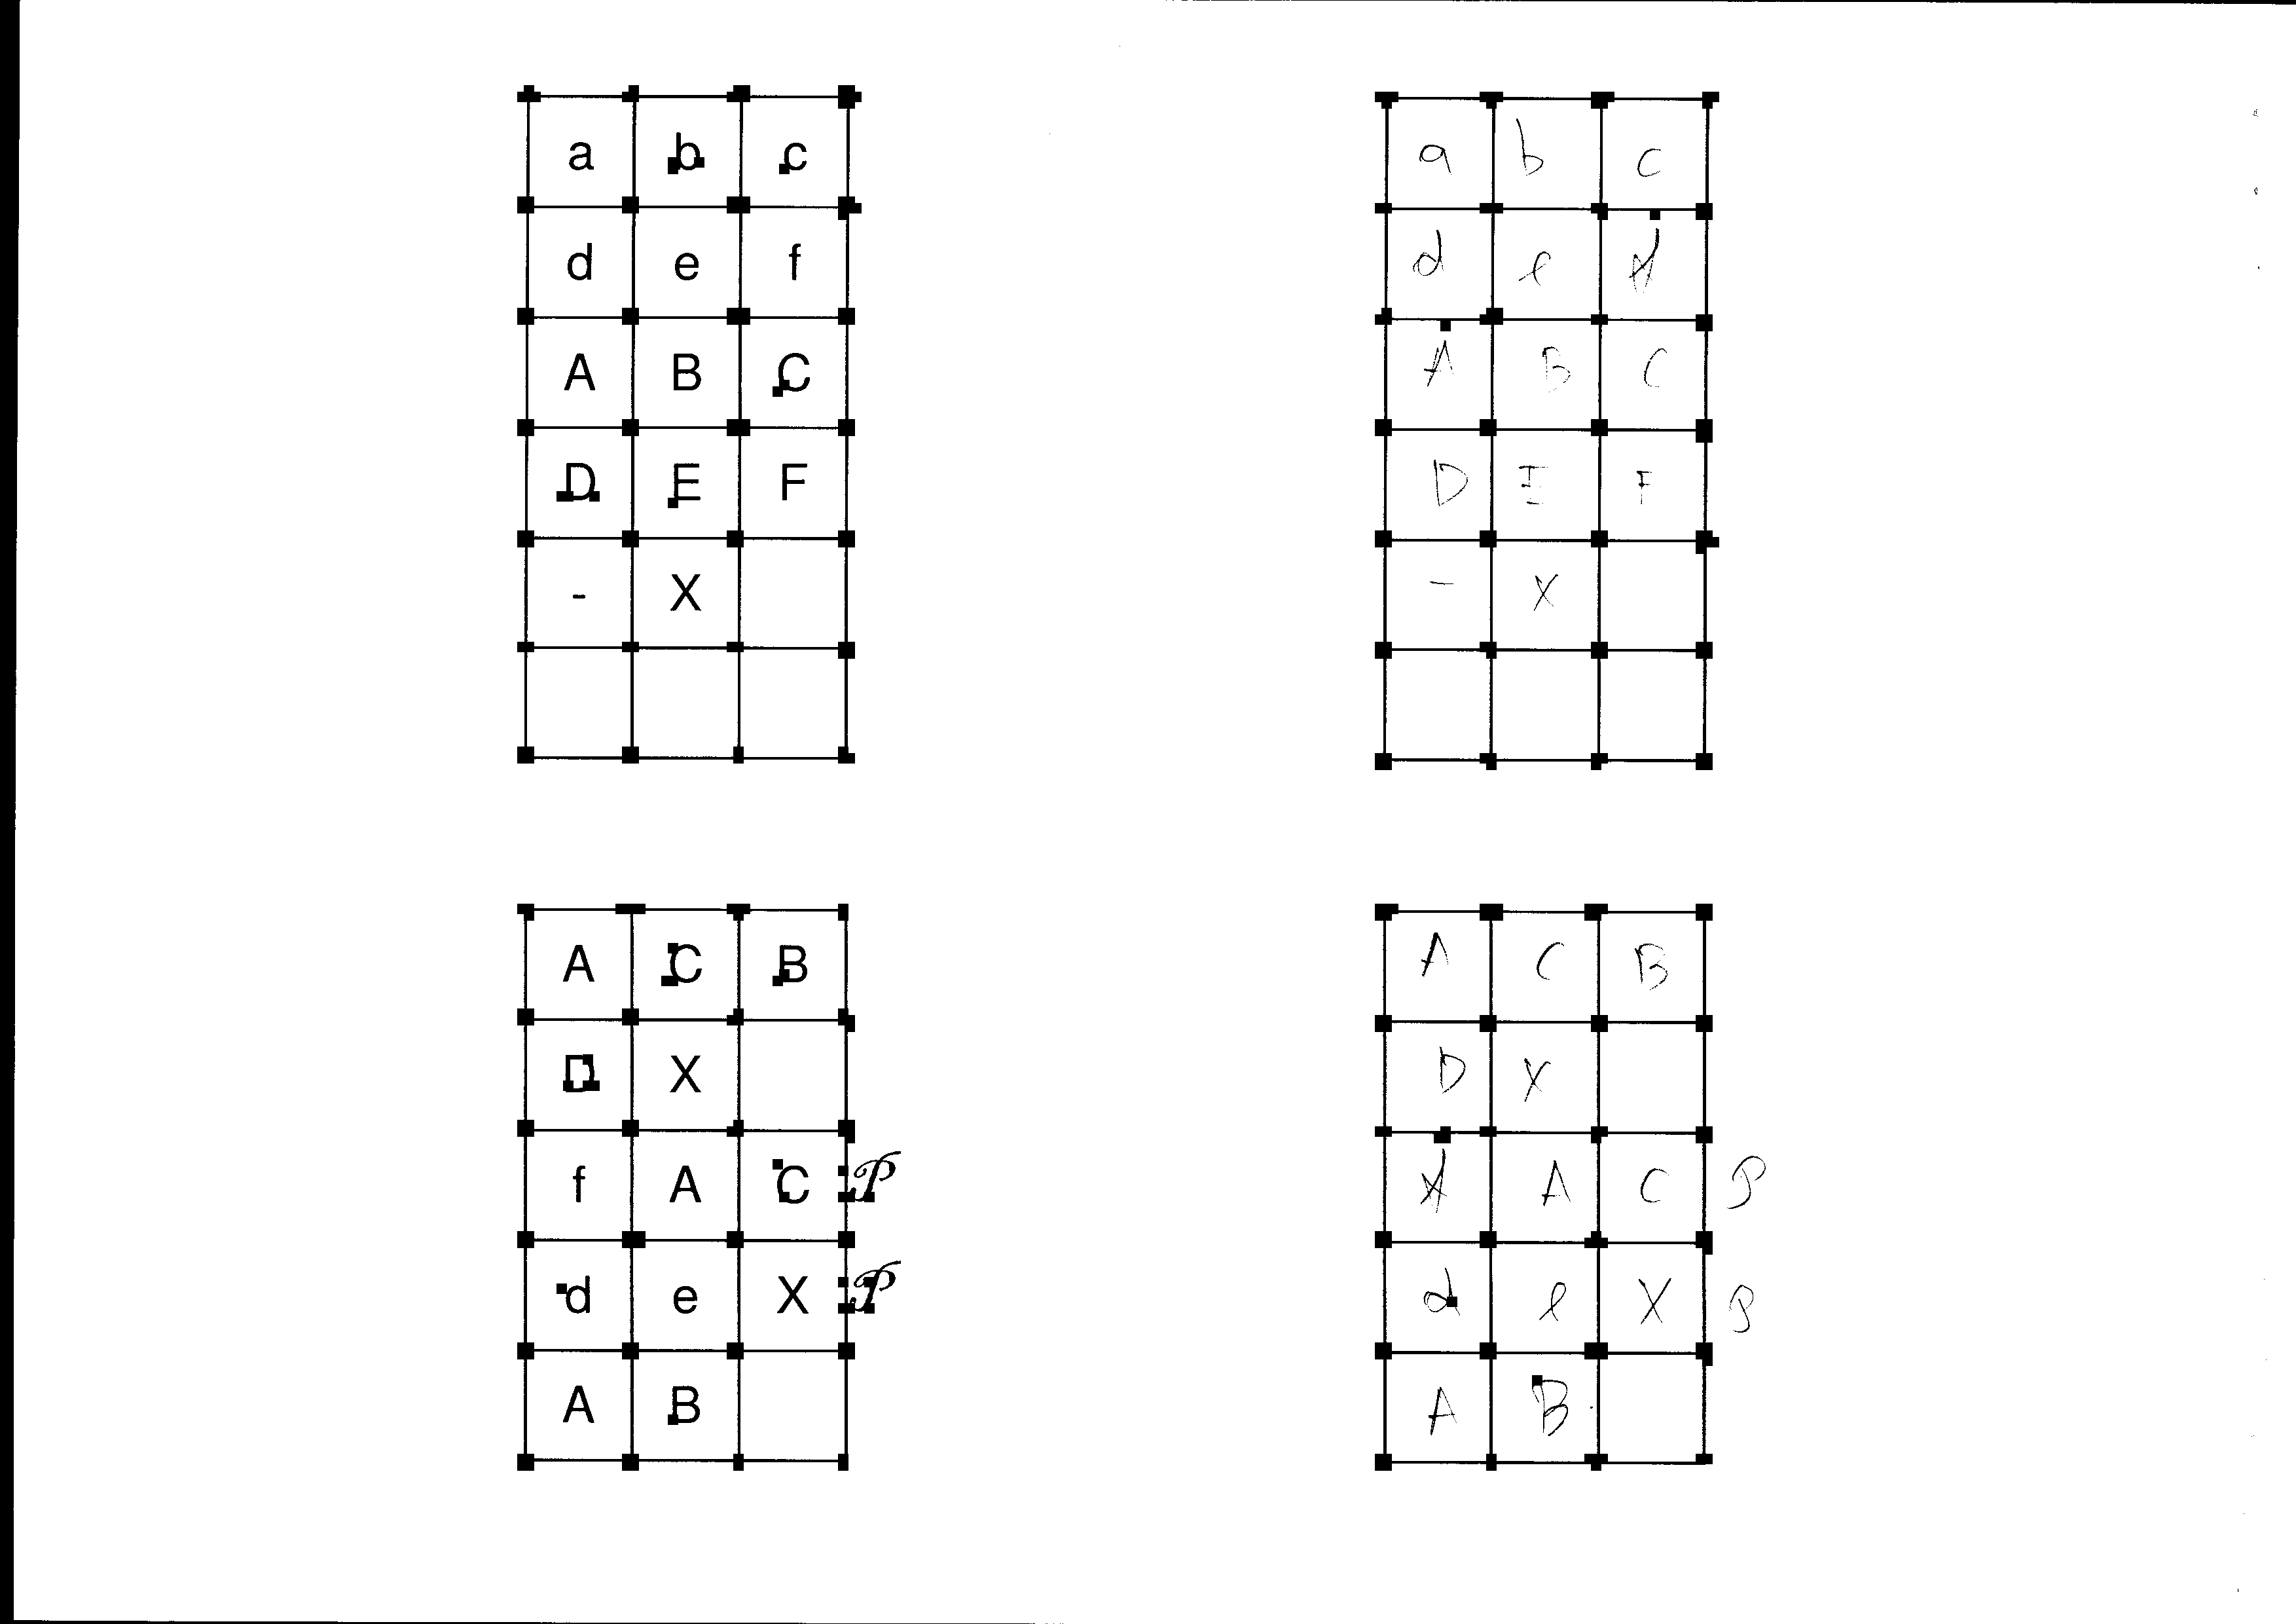
\includegraphics[width=.75\linewidth]{Images/combined.png}}
    \captionsetup{justification=centering}
    \caption{Točke detektirane korištenjem kombinacije algoritma AdaBoost i umjetne neuronske mreže}
    \label{fig:combinedResult}
\end{figure}

Slika \ref{fig:combinedResult} prikazuje rezultat dobiven korištenjem oba prethodno opisana klasifikatora, na način kakav je prethodno objašnjen.
Primjećuje se kako su sve točke od interesa i dalje prepoznate, no svejedno postoji manji broj točaka koje nisu trebale biti prepoznate.
Valja uočiti kako su sve stvarne točke od interesa prepoznate nekoliko puta, što je kasnije iskorišteno kako bi se maknule lažno prepoznate točke.\\

Algoritam je pokrenut na $10$ primjera veličine $3507x2480$ slikovnih elemenata te su zabilježena sljedeća vremena izvođenja: $423.615$, $415.388$, $397.672$, $417.765$, $446.087$, $396.153$, $403.633$, $414.420$, $416.799$, $407.353$, izraženo u milisekundama. 
Prosječno vrijeme izvođenja iznosi $413.9$ms.\\

Primjenom T-testa uz hipoteze $H_0: \mu_1 = \mu_2$ i $H_1: \mu_1 < \mu_2$, gdje je sa $\mu_1$ označeno prosječno vrijeme izvođenja klasifikatora dobivenim korištenjem algoritma AdaBoost i neuronske mreže, a sa $\mu_2$ klasifikator koji koristi isključivo neuronsku mrežu.
Dobivena je $P$ vrijednost $2.979\cdot10^{-9}$ na temelju čega se uz nivo značajnosti $\alpha = 0.05$   hipoteza $H_0$ odbacuje u korist hipoteze $H_1$ čime se zaključuje kako je prosječno vrijeme izvođenja klasifikacije kombinacijom algoritma AdaBoost i umjetne neuronske mreže statistički značajno manje od prosječnog vremena izvođenja klasificiranja korištenjem isključivo umjetne neuronske mreže.

\subsection{Detekcija tablice}
Na temelju prepoznatih točaka vrhova ćelija potrebno je odrediti stvarnu tablicu.
Pri tome postoji nekoliko problema: svaki vrh je prepoznat više puta, postoje točke koje nisu vrhovi ćelija, potrebno je odrediti kako su vrhovi međusobno povezani.\\

Prvi isprobani pristup temelji se na pronalaženju grupe točaka unutar određenog radiusa te postavljanje stvarne točke na poziciju određenu aritmetičkom sredinom tih točaka.
Točke koje ne predstavljaju stvarni vrh ćelije detektiraju se tako što se nalaze same bez okolnih točaka.
Drugi način odbacivanja točke radi se kada se unutar dozvoljenog radijusa oko točke nalaze dvije točke koje su međusobno jako razmaknute, što zapravo znači da se točka nalazi na sredini između $2$ stvarna kuta te su zbog toga unutar dozvoljenog radiusa uključene točke različitih vrhova.
Problem može nastupiti kada se krivo prepoznata točka nalazi u blizini stvarnog vrha, zbog čega se pozicija konačne točke pomiče u odnosu na stvarno poziciju.\\

Konačna rekonstrukcija tablice radi se sortiranjem preostalih točaka po jednoj, zatim po drugoj koordinati.
Pritom treba paziti da točke koje leže na istoj vodoravnoj liniji tablice ne moraju nužno imati jednake vrijednosti $y$ koordinata, zbog čega prilikom sortiranja treba zanemariti razlike manje od određene konstante.

\begin{figure}[!ht]
    \centering
    \frame{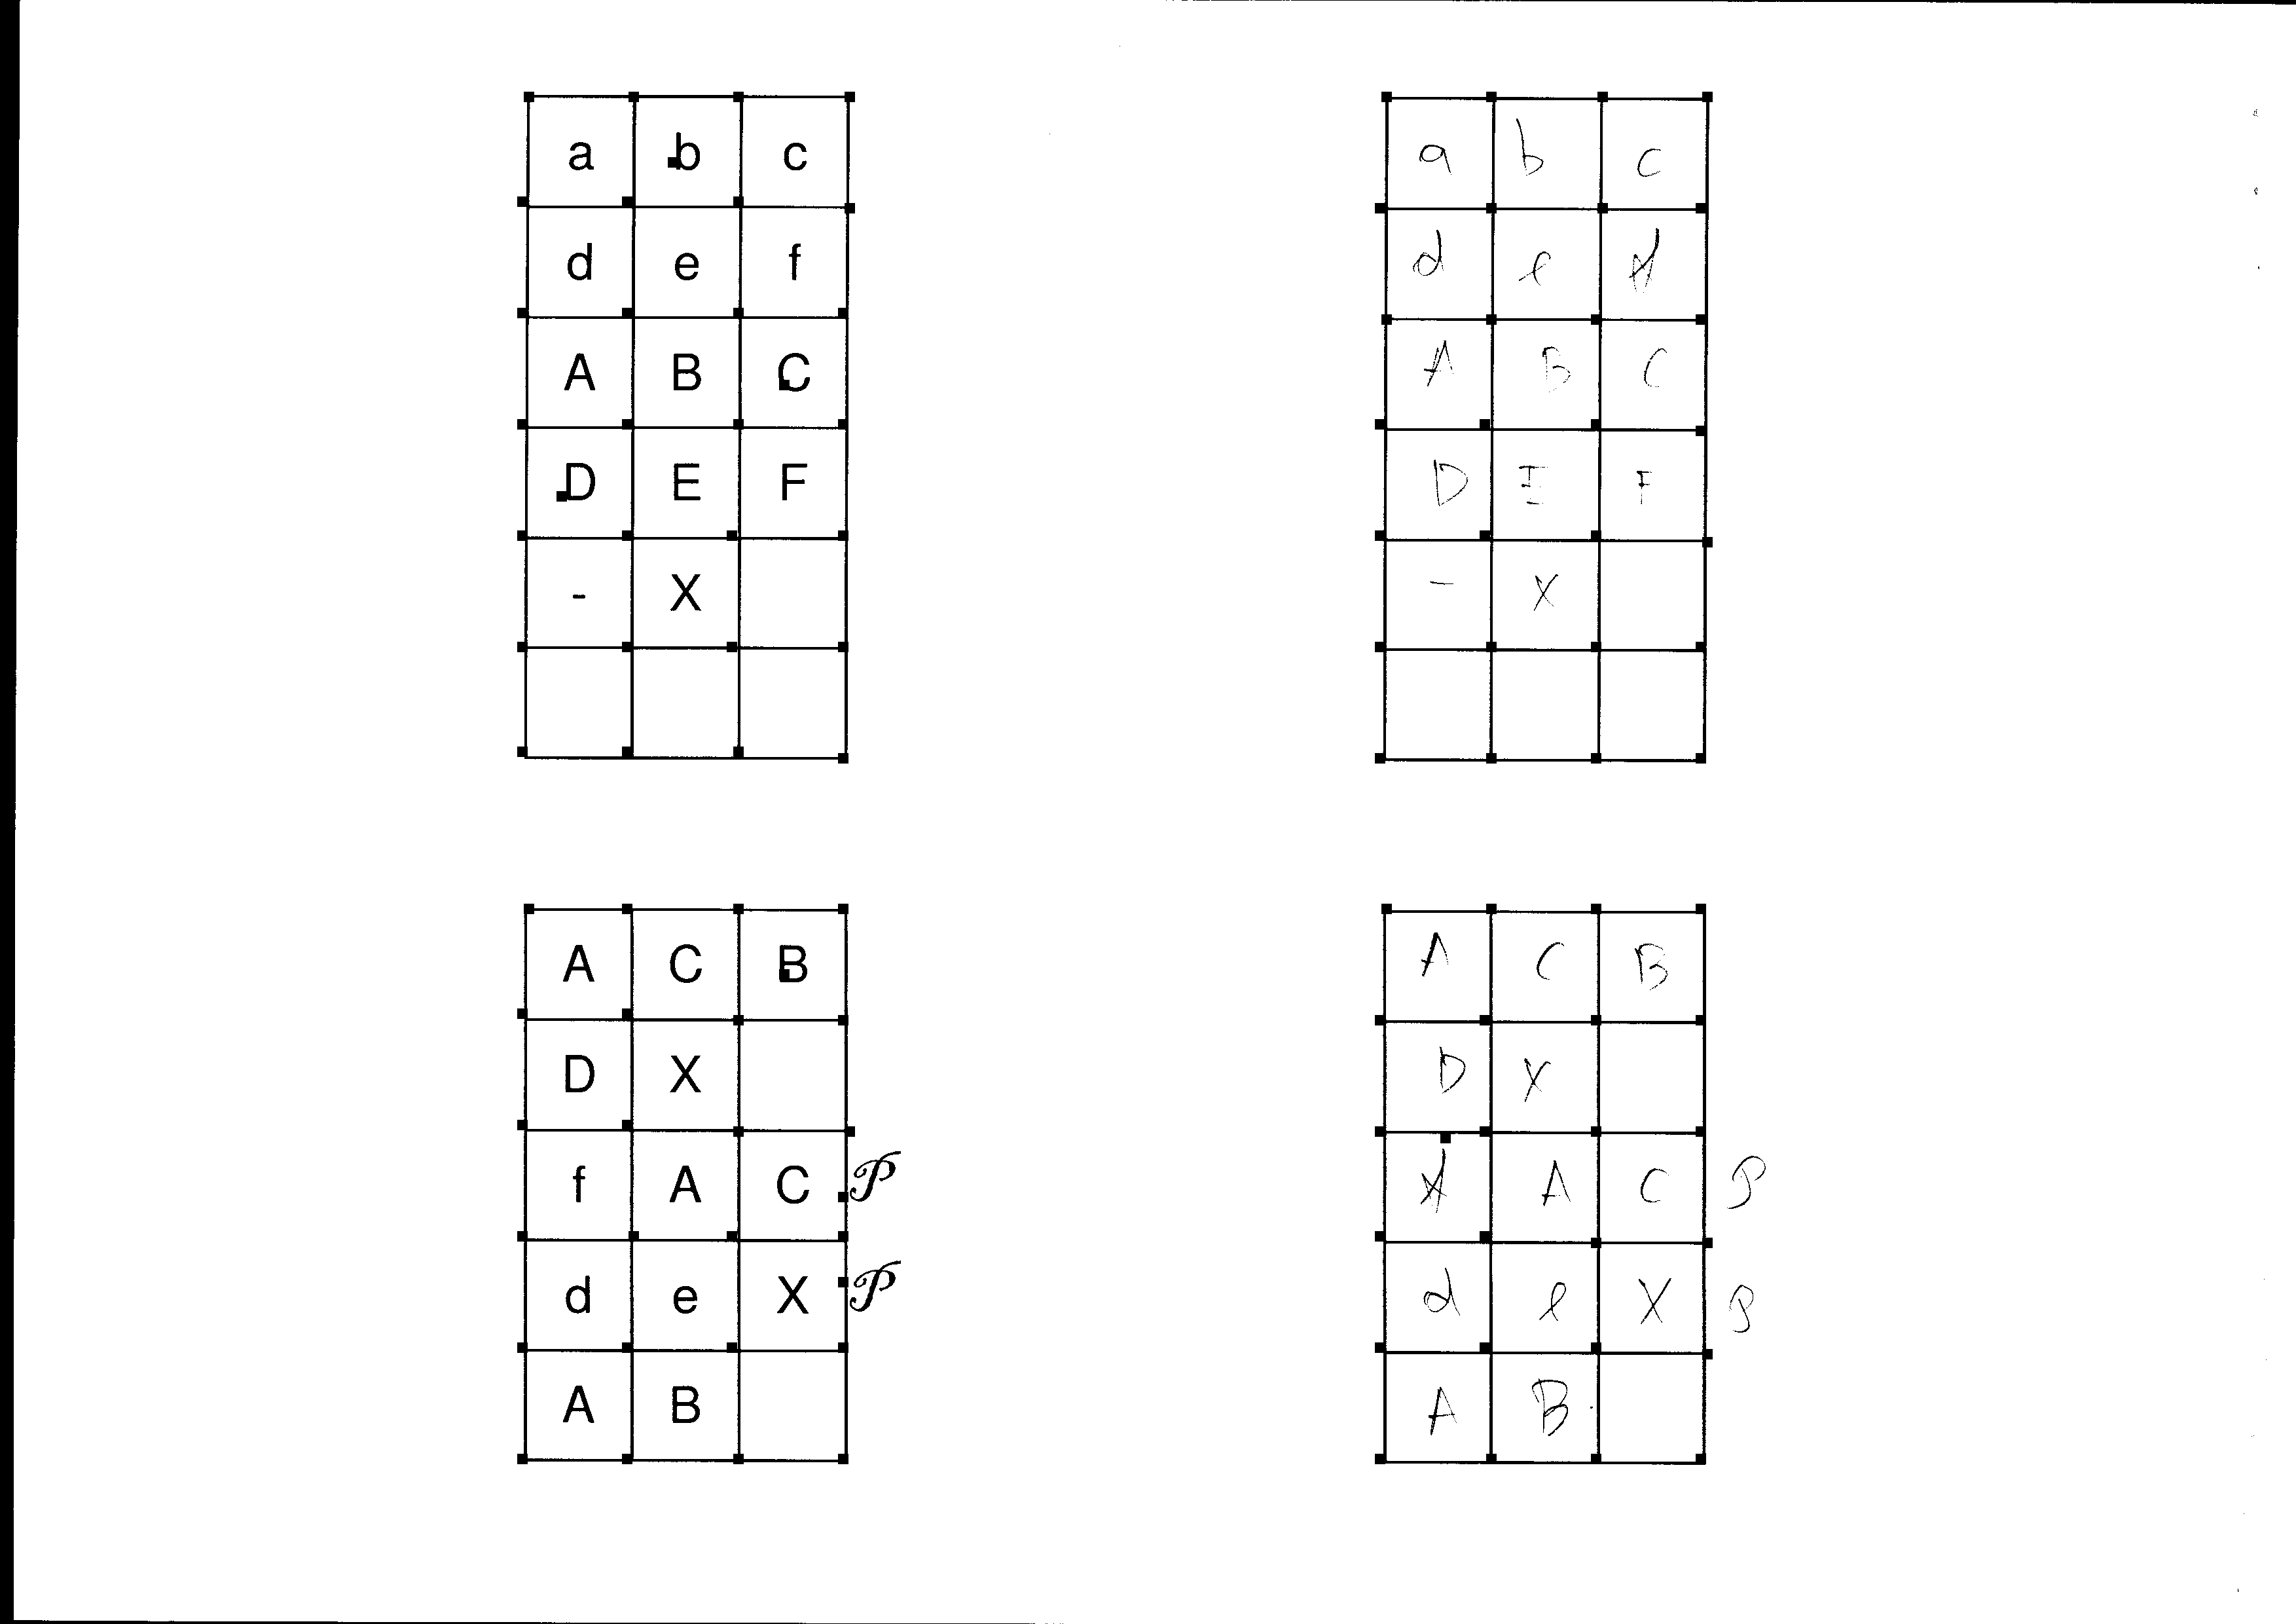
\includegraphics[width=.75\linewidth]{Images/tableV1.png}}
    \captionsetup{justification=centering}
    \caption{Primjer tablice prepoznate grupiranjem susjednih točaka}
    \label{fig:tableV1}
\end{figure}

Drugi korišteni način prikazan je na slici \ref{fig:tableV2}.
Tablica se prepoznaje tako da se naprave liste $x$ i $y$ koordinata prepoznatih točaka koje se potom sortiraju.
U sortiranim listama se traže grupe vrijednosti te se računa aritmetička sredina svake grupe kako bi se odredila $x$ odnosno $y$ koordinata svakog stupca odnosno retka tablice. 
Prilikom pronalaženja grupa vrijednosti provjerava se i broj pojavljivanja vrijednosti kako bi se izbacile točke koje se pojavljuju malo puta, odnosno koje su nastale greškom u klasifikaciji.\\

Rekonstrukcija tablice radi se tako da se na svaki mogući par $x$
i $y$ koordinata iz lista koordinata postavlja odgovarajući vrh ćelije.
Pri tome više ne postoji mogućnost da točke na istoj liniji imaju različite koordinate, što predstavlja problem u slučaju rotacije slike.
Dodatna limitacija ovog pristupa je korištenje pretpostavke da sve tablice imaju jednak broj ćelija u svakom retku, čime se gubi mogućnost spajanja ćelija ili tablica čiji vanjski obrub nije kvadratnog oblika.
Unatoč tome, u radu je korišten ovaj način rekonstrukcije tablice jer se pokazao robusnijim u odnosu na prepoznavanje grupa točaka za svaki vrh, a tablice nad kojima se algoritam koristi zadovoljavaju dodatne restrikcije ovog pristupa.\\

\begin{figure}[ht!]
    \centering
    \frame{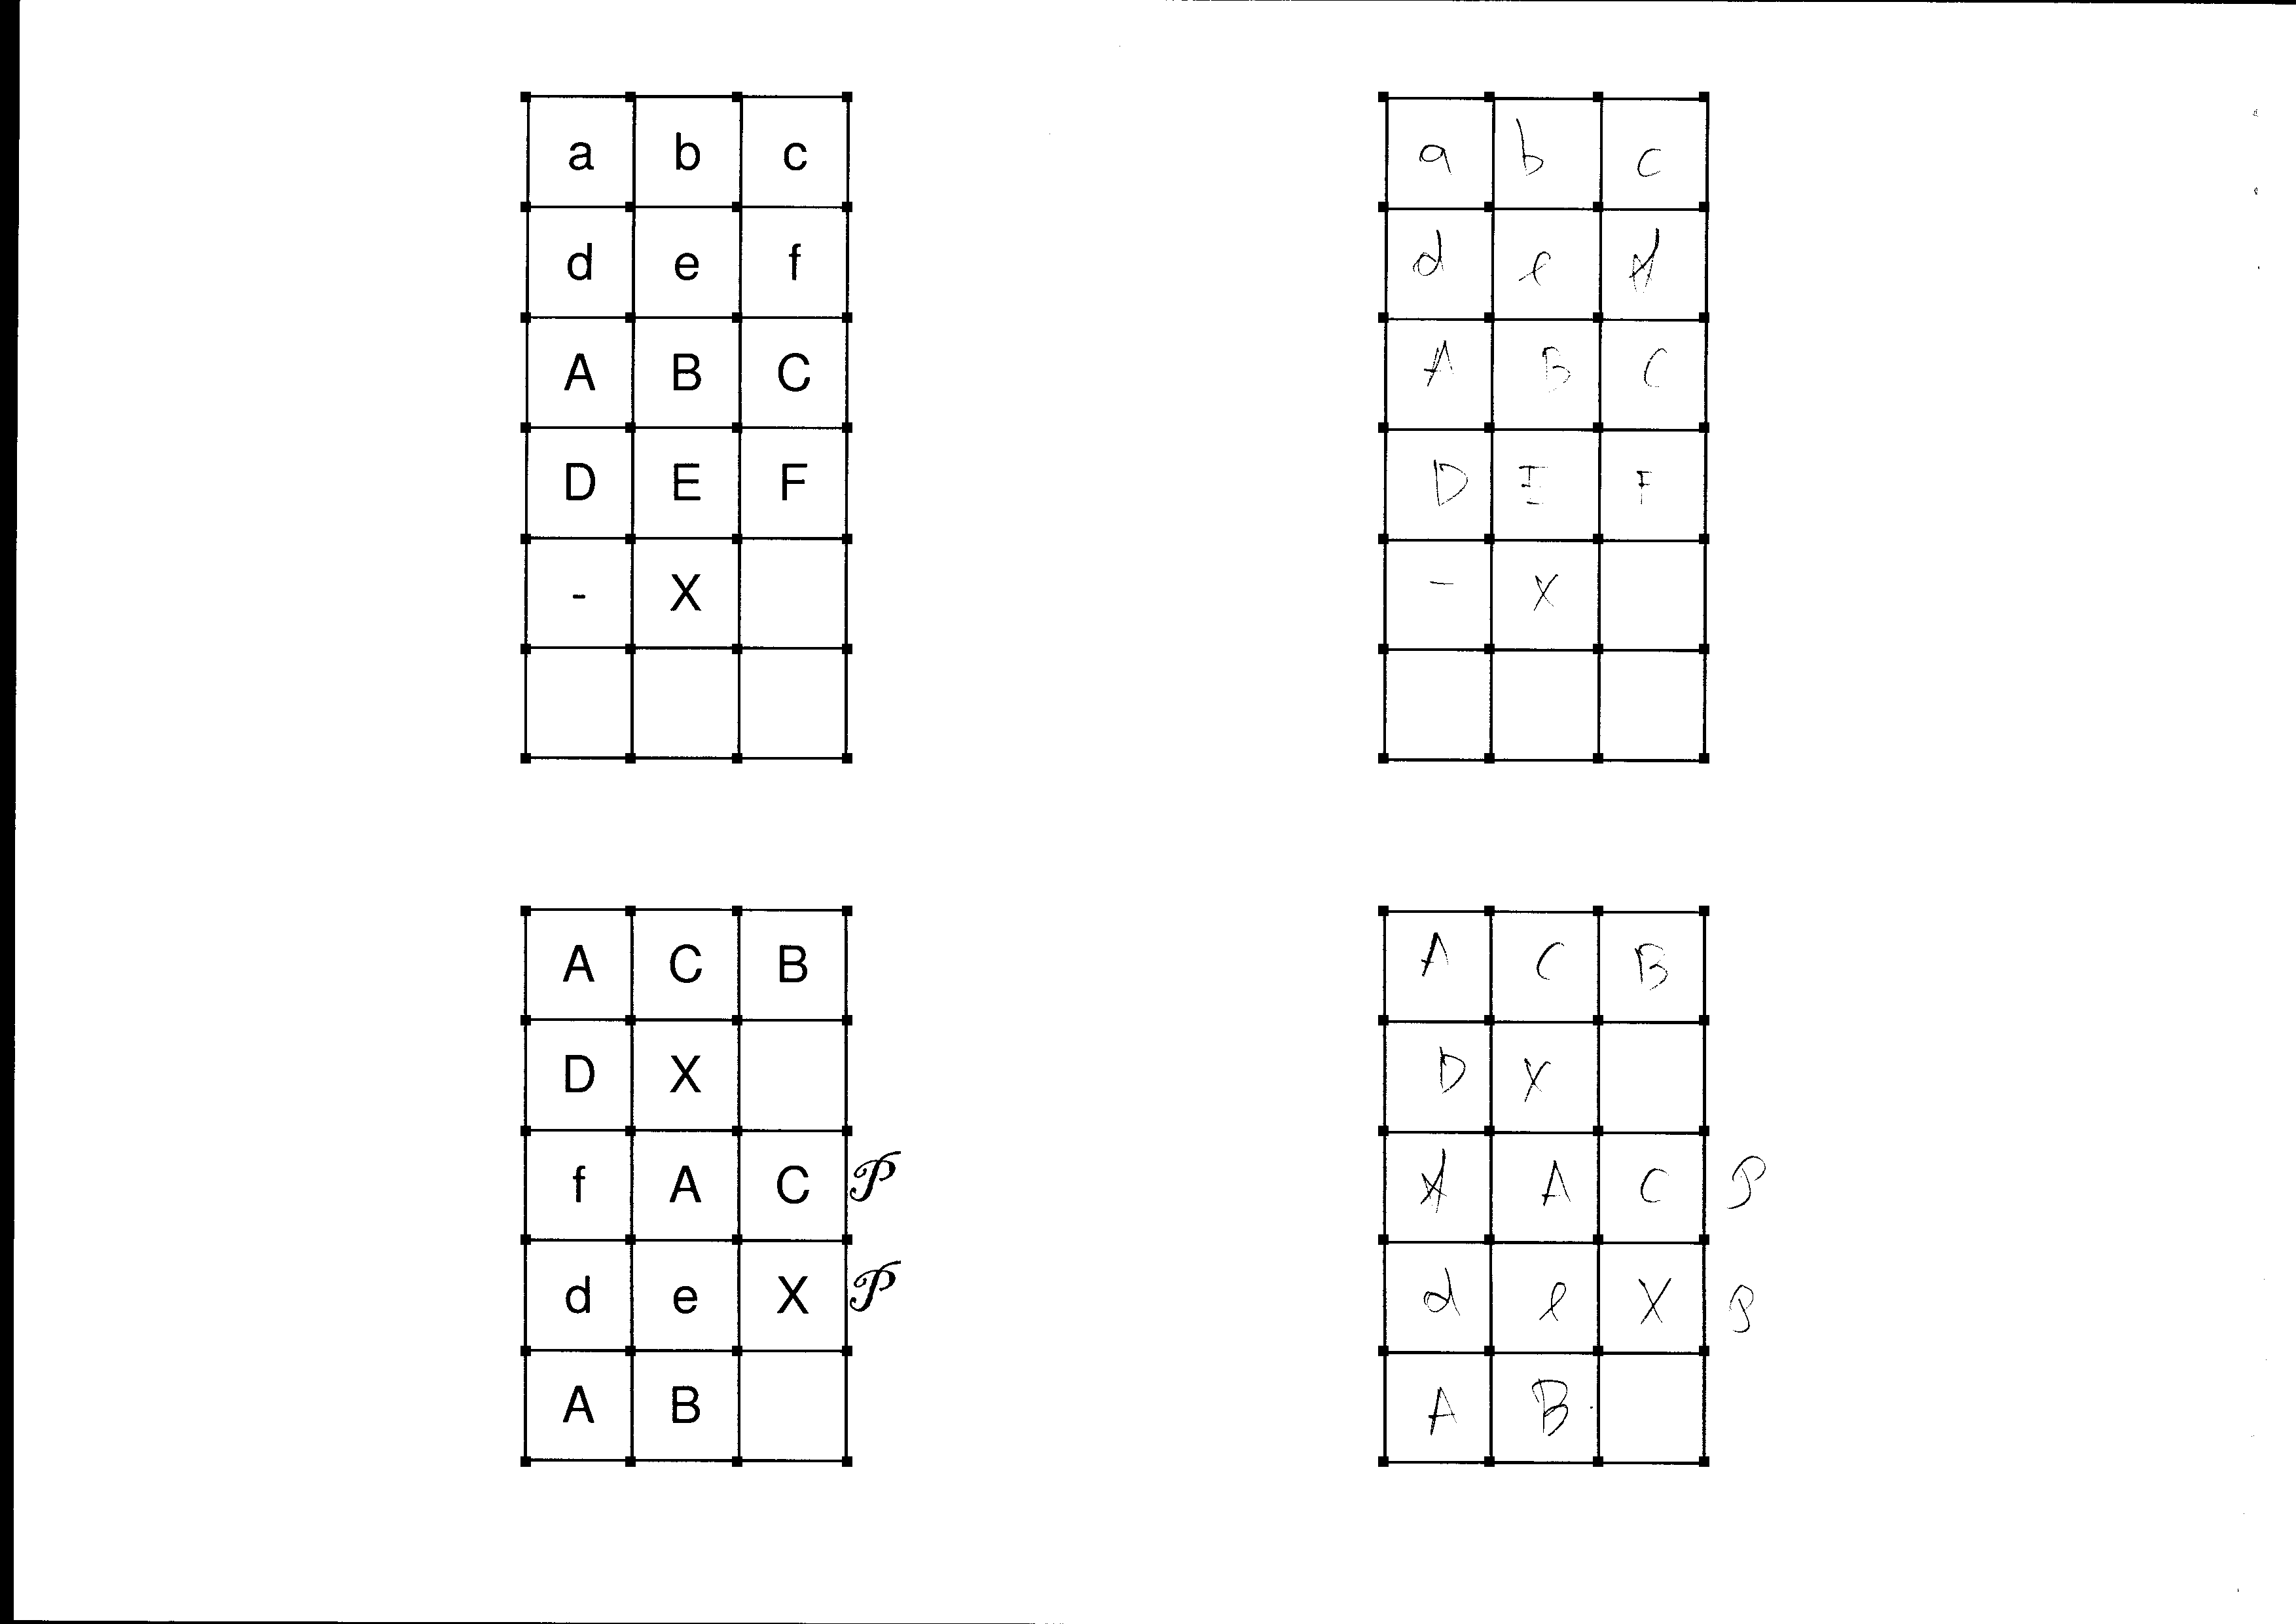
\includegraphics[width=.75\linewidth]{Images/tableV2.png}}
    \captionsetup{justification=centering}
    \caption{Primjer tablice prepoznate grupiranjem točaka po retcima i po stupcima}
    \label{fig:tableV2}
\end{figure}

Konačan algoritam pokrenut je na $4$ skupa tablica.
U prvom skupu uspješno je prepoznato $635/635$ tablica za što je bilo potrebno $13981.90$ms, odnosno prosječno $22.02$ms po tablici, pritom u navedeno vrijeme nije ubrojeno vrijeme učitavanja slike s diska niti vrijeme spremanja rezultata na disk.
U drugom skupu uspješno je prepoznato $362/362$ tablica za što je bilo potrebno $11584.47$ms, odnosno prosječno $32.00$ms po tablici.
U trećem skupu uspješno je prepoznato $685/685$ tablica za što je bilo potrebno $25604.96$ms, odnosno prosječno $44.17$ms po tablici.
U četvrtom skupu uspješno je prepoznato $580/580$ tablica za što je bilo potrebno $21010.13$ms, odnosno prosječno $36.22$ms po tablici.
Valja napomenuti kako ovi rezultati ne znače da je svaka ćelija točno određena, već su moguća manja odstupanja.\\

Korištenjem postupka detekcije koji koristi prethodno stečeno znanje kao što je prethodno bilo opisano dobiveni su sljedeći rezultati.
U prvom skupu uspješno je prepoznato $635/635$ tablica za što je bilo potrebno $7779.37$ms, odnosno prosječno $12.25$ms po tablici..
U drugom skupu uspješno je prepoznato $362/362$ tablica za što je bilo potrebno $6157.72$ms, odnosno prosječno $17.01$ms po tablici.
U trećem skupu uspješno je prepoznato $650/685$ tablica za što je bilo potrebno $13174.98$ms, odnosno prosječno $19.23$ms po tablici.
U četvrtom skupu uspješno je prepoznato $578/580$ tablica za što je bilo potrebno $10059.67$ms, odnosno prosječno $17.34$ms po tablici.
Primjećuje se kako je u ovom slučaju točnost prepoznavanja tablica smanjena.
Točnost uvelike ovisi i o selekciji referentne tablice prilikom prepoznavanja daljnjih tablica, te je ovdje uvijek korištena prva tablica iz skupa podataka.
Podatci iz trećeg skupa ponovno su detektirani korištenjem drugačije odabrane referentne tablice, što je rezultiralo točnošću od $680/685$ ispravno prepoznatih tablica.
Navedeni problem moguće je riješiti ponovnom detekcijom tablice, bez korištenja prethodno stečenog znanja za slučajeve u kojima se tablica krivo prepoznala.
Takve slučajeve lako je programski prepoznati jer sadrže manji broj pronađenih vrhova ćelija od onoga koji je očekivan.\\


\chapter{Zaključak}
\label{ch:conclusion}
Ovaj rad analizira različite pristupe detekcije tablica na skeniranim dokumentima, sa svrhom primjene u automatizaciji ispravljanja pismenih ispita.
Isprobani su različiti načini binarizacije slike kao i obrade iste prije početka detekcije te je ustanovljeno kako nije potrebno koristiti adaptivnu binarizaciju.
Postupak detekcije podijeljen je na postupak detekcije vrhova ćelija i na rekonstrukciju tablice iz pronađenih vrhova.
Detekcija i klasifikacija ćelija radi se korištenjem unaprijedne umjetne neuronske mreže, koja kao ulaze dobiva elemente koje je klasifikator temeljen na algoritmu AdaBoost prepoznao kao potencijalne vrhove.
Na taj je način dobiven konačan klasifikator koji nakon što se jednom istrenira radi brzo nad novim ulaznim slikama.
Konačna rekonstrukcija tablice testirana je nad skupom od preko $2000$ tablica te se pokazala uspješnom.



\bibliography{literatura}
\bibliographystyle{fer}

\begin{sazetak}
Problem očitavanja sadržaja skeniranih dokumenata javlja se u mnogim područjima ljudskoga rada.
Automatizacija tog postupka može značajno smanjiti vrijeme koje se troši na ručno očitavanje. 
Problem se pri tome može razložiti na niz potproblema, ovisno o strukturi informacija koje su prisutne u dokumentu.\\

U okviru završnog rada istraženi su i opisani postupci precizne detekcije tablica. 
Detektiran je položaj tablice te je ponuđena mogućnost izolirana svake od ćelija tablice, kako bi se njihov sadržaj potom mogao obraditi nekim drugim postupkom.
Pri tome treba je moguće da se u okolini tablice nalaze različite smetnje te da ćelije tablice budu popunjene različitim sadržajima. 
Razvijeno je programsko rješenje koje korištenjem klasifikatora temeljenog na algoritmu AdaBoost i klasifikatora pomoću unaprijedne umjetne neuronske mreže uspješno prepoznaje tablice.


\kljucnerijeci{detekcija tablica, ekstrakcija ćelija, prepoznavanje objekata, klasifikacija}
\end{sazetak}

\engtitle{Table Extraction on Scanned Documents}
\begin{abstract}
The problem with reading content from scanned documents occurs in many areas of human activities.
Automation of this process can significantly reduce the time that is spent on manual readings.
This problem can be broken down into a series of subproblems, depending on the structure of the information that is present in the document.\\

This thesis researches and describes algorithms for precise table detection.
The position of the table is beeing detected, and the possibility of extracting the content of each individual cell is offered, so that it can be used for further detection.
It is possible for the document to contain various interferences within the region of the table, and that table cells are filled with a variety of content.
The developer software solution, that uses a classifier based on the AdaBoost algorithm and a classifier based on feedforward artificial neural networks, successfully identifies the table on given grayscale images.

\keywords{table detection, cell extraction, object detection, classification}
\end{abstract}

\end{document}
